% =====================================================================
%  AI-Driven Gaming Addiction Screening System
%  PES University Capstone -- PW26_SAS-03  (UE23CS320B, Phase-2)
%
%  This paper describes the system AS ACTUALLY BUILT (native Android apps +
%  cloud Flask backend + calibrated classical-ML ensemble). Metrics reported
%  here are the honest, current numbers from model_metadata.json.
%
%  Compile:  pdflatex PROJECT_PAPER.tex   (twice, for the ToC/refs)
% =====================================================================
\documentclass[11pt,a4paper]{article}

\usepackage[T1]{fontenc}
\usepackage[utf8]{inputenc}
\usepackage[margin=1in]{geometry}
\usepackage{booktabs}
\usepackage{tabularx}
\usepackage{xltabular}   % tabularx X-columns that break cleanly across pages (revision table)
\usepackage{tikz}
\usetikzlibrary{positioning, arrows.meta, fit, backgrounds, calc}
\usepackage{amsmath}
\usepackage{newtxtext}   % dark, readable Times text (replaces thin Computer Modern)
\usepackage{newtxmath}   % matching math font; keeps real subscripts in formulae
\usepackage{enumitem}
\usepackage{xcolor}
\usepackage{listings}
\usepackage{caption}
\usepackage{graphicx}
\usepackage[hidelinks]{hyperref}
\usepackage{microtype}   % char protrusion + font expansion: far fewer words run off the margin
\usepackage[strings]{underscore}  % printable underscores in text; subscripts still work in math

\setlength{\parskip}{0.45em}
\setlength{\parindent}{0pt}
\setlength{\emergencystretch}{3em}  % last-resort stretch so lines don't overflow the right margin

% Compact, build-safe capability marks for the comparison table (avoid amssymb /
% \part clash). \capY = yes, \capP = partial, \capN = no.
\newcommand{\capY}{\textcolor{green!50!black}{\textbf{Y}}}
\newcommand{\capP}{\textcolor{orange!90!black}{\textbf{P}}}
\newcommand{\capN}{\textcolor{black!45}{\textbf{--}}}

\lstset{
  basicstyle=\ttfamily\footnotesize,
  breaklines=true,
  frame=single,
  columns=fullflexible,
  keepspaces=true,
  showstringspaces=false,
  xleftmargin=0.5em,
}

\title{\textbf{AI-Driven Gaming Addiction Screening System}\\
\large A Multimodal, Privacy-Conscious Mobile Platform for Early
Detection and Parental Awareness}

\author{
Kaustubh Agarwal (PES1UG23CS291) \and
Khushee P Kiran (PES1UG23CS303) \and
Kanak Goyal (PES1UG23CS279) \and
Vidisha Murali (PES1UG23CS681) \\[0.5em]
\textit{Under the guidance of Prof. Shridevi Sawant} \\
\textit{Department of Computer Science and Engineering, PES University} \\
\textit{Capstone Project PW26\_SAS-03 (UE23CS320B), January--May 2026} \\
\textit{(live family pilot and evaluation continued through August 2026)}
}
\date{}

\begin{document}
\maketitle

% ---------------------------------------------------------------------
\begin{abstract}
\noindent
Excessive mobile gaming is increasingly linked to disrupted sleep, mood and
routine in adolescents, yet most existing tools track only raw screen time and
miss the patterns that distinguish healthy play from problematic use. We present
a deployed, multimodal screening platform that fuses three signals collected
during real gameplay --- objective play behaviour, in-game chat toxicity, and
voice emotion --- into a single risk band (Casual / At-Risk / Addicted; surfaced
to families as Low / Some / High concern), with the behaviour and chat
probabilities isotonic-calibrated. Two native Android applications (a Child
monitoring app and a Parent dashboard) talk to a cloud Flask backend serving a
weighted ensemble of three classical machine-learning models, favoured \emph{a
priori} over deep alternatives for SHAP explainability, free-tier cloud
deployability, and a privacy design that reduces raw media to compact features
and deletes it. Within that class, every model-family choice is backed by a measured bake-off,
feature and corpus choices by ablations with bootstrap confidence intervals, and
the fusion priors by sensitivity analyses on live pilot decisions. The pipeline
is grounded in \emph{eleven real, open datasets}: the chat model reaches $0.96$
precision at its alert threshold on held-out real gaming chat, detects
code-mixed Hinglish/Devanagari abuse whether typed or \emph{spoken} (transcribed
on-device; uploaded audio is deleted after feature extraction) --- with the
Hindi path \emph{trained and held-out-validated} on the HASOC 2019 corpus in
both scripts, Devanagari and colloquial romanisation ($\geq$$0.95$ precision at
the alert threshold on each, from near-zero model coverage before adoption); the voice model
is trained on $9{,}817$ real speech clips across $154$ ingested speakers in
three languages and evaluated speaker-independently; play-time distributions and
peer percentiles follow a real survey of $13{,}464$ gamers; and an
$11{,}191$-respondent IGDS9-SF dataset validates the severity base rate and the
chat channel's core premise. The production deployment (HTTPS, token
authentication, versioned parental consent) ships a parent-feedback loop that
turns accurate/false-alarm verdicts into measured threshold recommendations, a
drift monitor, and a parent-to-child nudge channel; a consented live family
pilot has exercised every capture channel and alert type in production.
Critically, the risk score is then validated \emph{externally}: in an anonymous
adult survey ($134$ raw, $104$ usable), the score the system would have served
correlates with the clinically-validated IGDS9-SF instrument at Spearman
$\rho = 0.317$ ($95\%$ CI $[0.137, 0.478]$), leads the self-reported
screen-time baseline it is meant to replace in $97.4\%$ of paired resamples
($\Delta\rho = +0.167$), and survives partialling that baseline out
($\rho = 0.303$, CI excluding zero), with the signal concentrated in the
behavioural-pattern features rather than the volume ones --- the project's core premise, confirmed
against real labels rather than assumed. Remaining limits are stated plainly ---
behavioural \emph{labels} remain synthetic screening priors, so caseness
metrics at the clinical cut-off are still uncomputed, and one ensemble component
(genre weighting) failed to reach significance --- and the output is framed
explicitly as \emph{screening and awareness, not clinical diagnosis}.
\end{abstract}

\tableofcontents
\vspace{1em}

% =====================================================================
\section{Introduction}
% =====================================================================
Mobile gaming is now a daily activity for most adolescents. While gaming is not
inherently harmful, a minority of users develop patterns that the DSM-5 (Internet
Gaming Disorder) and ICD-11 (Gaming Disorder) characterise behaviourally: impaired
control over play, escalating priority of gaming over other activities, and
continuation despite negative consequences. Conventional parental-control tools
report \emph{how long} a phone was used but not \emph{how} the child played --- the
late-night sessions, the rapid re-logins, the rising frustration in chat and voice.

This project builds a system that captures those richer signals during gameplay and
turns them into an interpretable risk band that a parent can act on with
\emph{awareness rather than punishment}. Our key design stance is honesty and
deployability: every claim in this paper reflects the system as actually built and
running, and the models are chosen to be lightweight, explainable, and calibrated
rather than to maximise a headline accuracy number.

\subsection*{Contributions}
\begin{enumerate}[leftmargin=1.4em]
  \item A deployed three-tier platform: two native Android apps + a cloud Flask
        backend serving a multimodal ML ensemble.
  \item A behavioural feature pipeline that computes ten \emph{measured} features
        from real session history; the model is trained on these ten alone, while ten
        psychometric proxies --- derived through a \emph{single shared function} ---
        serve as parent-facing explanations. This eliminates train/serve skew and
        keeps SHAP attributions non-circular (\S\ref{sec:features}).
  \item An availability-weighted ensemble that re-normalises over only the
        modalities that produced data, with isotonic probability calibration and
        per-prediction SHAP explanations.
  \item Production engineering: token authentication, peppered PIN hashing,
        HTTPS-only transport, encrypted on-device token storage, parental consent,
        raw-audio deletion, and a durable managed database --- plus free-tier load
        engineering (pooled, validated connections to the serverless database,
        per-client rate limiting behind the reverse proxy, and caching/throttling on
        the polling hot paths) so the deployment survives real concurrent use.
        Privacy rights are engineered symmetrically: data \emph{export} and data
        \emph{deletion} share one table inventory in code, so ``show me everything you
        hold'' and ``erase everything you hold'' can never silently drift apart; and a
        scheduled drift monitor compares each week's served score distributions against
        a reference window (PSI/KS) directly on the production database, so the
        deployed models are \emph{watched}, not just shipped.
  \item A parent-feedback loop that records real ``accurate / false-alarm''
        verdicts --- the only source of genuine labels in an otherwise
        synthetically-trained system --- enabling future retraining.
  \item A parent-to-child nudge channel (preset or custom messages, plus an automatic
        ``mind the language'' nudge on toxic chat) that turns the platform from passive
        monitoring into two-way guidance.
  \item A custom-keyboard (Input Method Editor) chat-capture path that reliably records
        the child's typed in-game text even in canvas/engine games (e.g.\ Roblox) the
        accessibility API cannot read --- without resorting to screen OCR --- while
        capturing only the child's own typing.
  \item An \textbf{India-ready abuse channel} for code-mixed gaming chat: a curated
        Hinglish lexicon (romanised Hindi \emph{and} Devanagari script; screened
        against the Bohra et al.\ code-mixed hate lexicon~\cite{bohra2018}, from
        which only unambiguous slur families were adopted --- generic negativity
        such as \emph{fake} or \emph{selfish} is precision-poison for an alerting
        channel) fused with the
        calibrated English toxicity model via noisy-OR --- a \emph{trained}
        dual-script Hindi path (HASOC 2019 in Devanagari \emph{and} colloquial
        romanisation: held-out alert precision $\geq$$0.95$ on both scripts where
        the pre-adoption model caught almost nothing, \S6.2 --- the trained rows
        now carry most of what the hand lexicon alone once provided) --- and an
        \emph{on-device} Indian-English speech-to-text path (Vosk) that routes what the
        child \emph{says} through the same toxicity model, so spoken \emph{English}
        abuse is caught without raw audio ever being retained (spoken \emph{Hindi}
        words remain outside the validated build --- a dual-recogniser mode is
        implemented but off by default, \S9). English-centric keyword monitors cover
        neither.
  \item Tamper resistance and resilient delivery: a self-restarting foreground service,
        a battery-optimisation exemption step (OEM power managers silently killing the
        monitor are the most common real-world failure), a parent-PIN lock on
        logout/settings with parent-role-only credential and data-deletion changes, a
        server-side heartbeat watchdog that alerts the parent when monitoring goes silent
        (uninstall / kill / offline), a live parent-dashboard indicator of monitoring
        health --- uptime, uninstall-protection, and \emph{capture-permission} status, so
        the parent sees when the app is running but degraded (e.g.\ accessibility revoked);
        revoking a capture permission also raises a one-shot push alert rather than only
        flipping the badge --- and ``playing right now'', an offline retry queue so chat captured
        without connectivity is delivered later instead of lost, and real-time alerts
        pushed to \emph{every} guardian device in a family.
  \item An evaluation methodology with teeth: model-family bake-offs for all three
        channels, one-component-at-a-time ablations with bootstrap confidence
        intervals, speaker-independent voice splits (which quantified a
        $\sim$9-point leakage inflation and \emph{reversed} a model-selection
        verdict), thresholds re-derived from held-out curves on every model change,
        and negative results reported alongside positive ones.
  \item \textbf{External construct validation against a clinical instrument}
        (\S\ref{sec:survey}). An anonymous adult survey ($134$ raw, $104$
        usable) paired the IGDS9-SF~\cite{igds9sf} with gaming-pattern questions
        scored through the \emph{deployed} serving path. The risk score tracks
        IGDS9-SF severity ($\rho = 0.317$, $95\%$ CI $[0.137, 0.478]$); it
        leads the self-reported screen-time baseline in $97.4\%$ of paired
        resamples ($\Delta\rho = +0.167$) and survives partialling that
        baseline out ($\rho = 0.303$, CI excluding zero); and the signal is
        carried by the five \emph{pattern} features, whose composite
        ($\rho = 0.330$) separates cleanly from the \emph{volume} composite
        ($\rho = 0.128$, CI including zero). The same
        study reports two results \emph{against} the system --- the genre
        multiplier reaches no significance, and four of five parent-facing
        psychometric proxies fail to track the IGDS item they are named after ---
        because a validation study that can only confirm is not one.
  \item Grounding in eleven real, open datasets (two behaviour-grounding surveys, five
        chat corpora, four speech corpora) --- each screened against explicit
        criteria, each adoption justified by a measured effect, and each rejection
        documented with its reason (\S4.2).
\end{enumerate}

% =====================================================================
\section{Related Work}
% =====================================================================
\textbf{AI-based monitoring of gaming disorder.} Reviews and cohort studies establish
that gaming disorder is multifactorial --- behavioural, emotional and
psychological~\cite{ergin2025,kaya2023} --- and that continuous, AI-based monitoring
detects early warning signs more reliably than self-report surveys or raw screen-time
tools~\cite{huang2024,jiang2024}. This motivates our continuous, multi-signal approach
and our behaviour-dominant weighting.

\textbf{Language and chat signals.} Short pieces of user text carry usable
addiction-risk and emotional signal~\cite{strojny2024}, and sentiment models perform
well on fast, informal, gaming-specific chat --- including multilingual
settings~\cite{kina2024}. This grounds our chat-toxicity channel and our future-work
direction of a multilingual/code-mixed model.

\textbf{Voice and multimodal fusion.} Combining speech with text yields stronger
emotional inference than any single stream~\cite{tyagi2024}, and acoustic cues (pitch,
energy, timbre) carry emotional information usable for behavioural
monitoring~\cite{schuller2013}. This supports our voice-emotion channel and the weighted
fusion of behaviour, chat and voice.

\textbf{On-device privacy and parental tools.} On-device processing supports
personalisation while keeping sensitive data on the phone~\cite{chakraborty2025}, and
prior work on parental-monitoring design stresses awareness and trust over
surveillance~\cite{iftikhar2021}; commercial tools such as Bark~\cite{bark2025} show
demand but are largely screen-time/keyword based. Such tools are also \emph{closed}:
their detection logic, thresholds and error rates are not published, so a parent
receives a flag with no stated basis and no way to judge its reliability. We position
our system as \emph{screening and guidance, not punishment}, with privacy-conscious
handling, per-prediction explanations, and a fully reproducible pipeline whose every
reported number traces to a runnable script.

\textbf{How our system differs.} Existing solutions fall into three groups, each with a
structural gap our platform closes. \emph{Screen-time / parental-control tools} (e.g.\
Google Family Link, built-in Digital Wellbeing) report \emph{how long} a phone is used
but nothing about \emph{how} the child plays. \emph{Keyword/heuristic monitors} (e.g.\
Bark~\cite{bark2025}) scan text for flagged words but model neither behavioural play
patterns nor chat inside canvas/engine games. \emph{Academic gaming-disorder
studies}~\cite{huang2024,jiang2024,strojny2024} demonstrate predictive signal but are
typically single-modality, offline, and evaluated on collected datasets rather than
shipped as a live, privacy-engineered system. Our contribution is the \emph{combination,
actually deployed}: (i)~a custom-keyboard (IME) path that captures the child's typed
in-game chat even in canvas games such as Roblox that the accessibility API cannot read,
without screen OCR; (ii)~an availability-weighted fusion of behaviour, chat and voice
into a single risk band, with isotonic-calibrated behaviour/chat probabilities and
SHAP-explained behavioural factors; (iii)~abuse detection built
for the \emph{Indian} gaming context --- code-mixed Hinglish and Devanagari text fused
with the calibrated English model, and spoken abuse transcribed \emph{on-device}
(Indian-English STT) into the same channel --- where keyword monitors are
English-centric; (iv)~a production-engineered, privacy-conscious two-app + cloud system
with tamper- and capture-permission health monitoring and two-way nudges (guidance, not
just alerts); and (v)~a realistic-stream evaluation with a live drift monitor,
so the deployed models are \emph{watched}, not merely shipped. Two cross-cutting
properties further separate the system from commercial tools: every risk band is
accompanied by a per-prediction, SHAP-based explanation --- the parent sees \emph{why},
not just a flag --- and the entire pipeline is reproducible, each reported metric
recomputable from an included script, where commercial detection logic is closed. The
novelty lies in this deployed, India-aware, explainable-and-audited combination and in
the canvas-game capture technique --- \emph{not} in the individual classical models,
which we deliberately keep lightweight and explainable. Table~\ref{tab:compare}
summarises the comparison. A fair-comparison caveat: the table compares
\emph{capability coverage}, not detection accuracy. Commercial tools publish neither
their models nor their error rates, and no shared benchmark exists, so no head-to-head
accuracy claim against them is possible --- and we make none. What we claim is the
combination of signals and properties they structurally do not offer, with our own
accuracy characterised in \S6 on open, reproducible evaluations.

\begin{table}[ht]
\centering
\small
\caption{Capability comparison with existing approaches
(\capY~= yes,\ \capP~= partial,\ \capN~= no).}
\label{tab:compare}
\begin{tabularx}{\linewidth}{@{}X *{4}{>{\centering\arraybackslash}p{1.85cm}}@{}}
\toprule
\textbf{Capability} & \textbf{Screen-time tools} & \textbf{Keyword monitors (Bark)} &
\textbf{Academic prototypes} & \textbf{Ours} \\
\midrule
Behavioural play-pattern signals (beyond duration)      & \capN & \capN & \capY & \capY \\
In-game chat capture                                    & \capN & \capY & \capP & \capY \\
Chat capture in canvas/engine games (Roblox), no OCR    & \capN & \capN & \capN & \capY \\
Code-mixed (Hinglish + Devanagari) abuse detection      & \capN & \capN & \capN & \capY \\
Spoken abuse caught via \emph{on-device} STT            & \capN & \capN & \capN & \capY \\
Voice-emotion signal                                    & \capN & \capN & \capP & \capY \\
Multimodal fusion into one risk band                    & \capN & \capN & \capP & \capY \\
Calibrated, SHAP-explainable output                     & \capN & \capN & \capP & \capY \\
Deployed end-to-end (apps + cloud)                      & \capY & \capY & \capN & \capY \\
Two-way guidance (nudges), not just alerts              & \capP & \capP & \capN & \capY \\
Tamper / capture-permission health awareness            & \capP & \capP & \capN & \capY \\
Deployed models monitored for drift (PSI/KS)            & \capN & \capN & \capN & \capY \\
Reproducible pipeline (open method, scripted metrics)   & \capN & \capN & \capP & \capY \\
Realistic-stream evaluation                             & \capN & \capN & \capP & \capY \\
\bottomrule
\end{tabularx}
\end{table}

% =====================================================================
\section{System Architecture with Explanation}
% =====================================================================
The platform follows a three-tier architecture (Fig.~\ref{fig:arch}):
a \textbf{data-collection tier} (Child app), a \textbf{serving tier} (Flask backend +
ML ensemble), and a \textbf{presentation tier} (Parent app).

\begin{figure}[h]
\centering
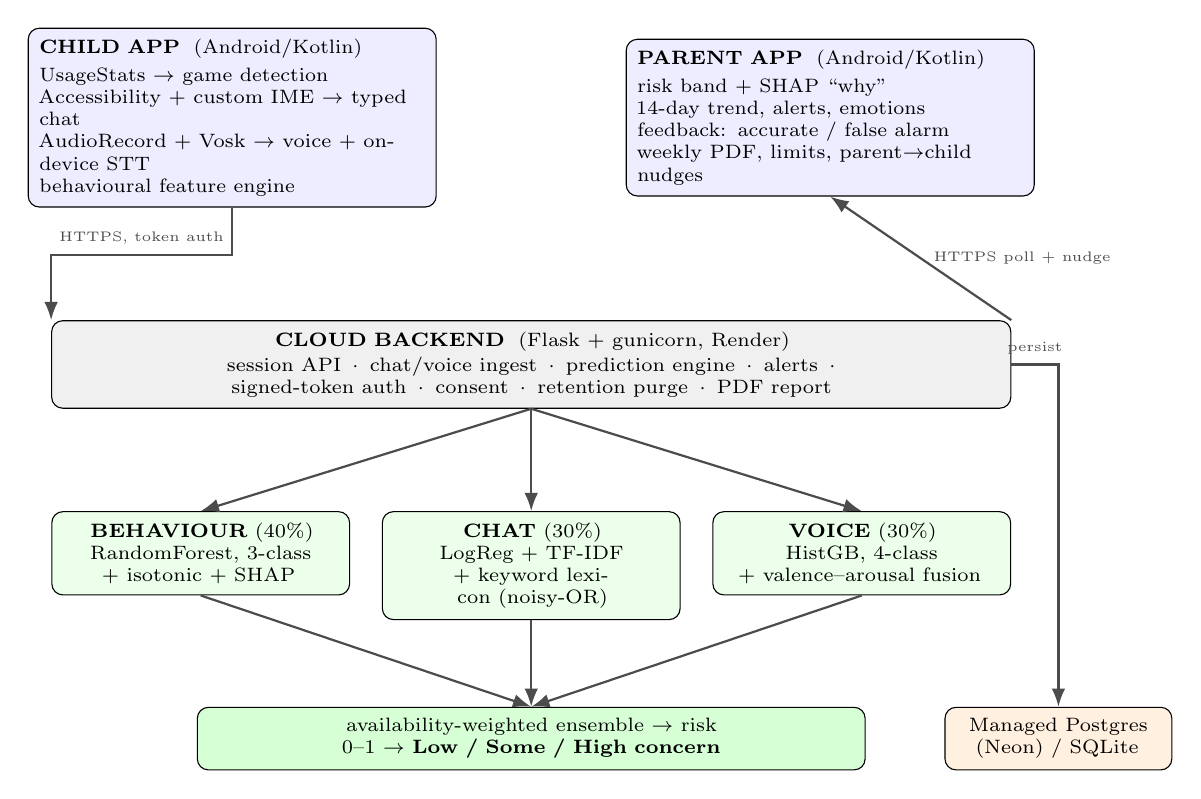
\begin{tikzpicture}[
  font=\scriptsize, >=Latex,
  box/.style={draw, rounded corners, align=left, inner sep=4pt, line width=0.4pt},
  app/.style={box, fill=blue!7, text width=4.9cm},
  cloud/.style={box, fill=black!6, text width=11.9cm, align=center},
  model/.style={box, fill=green!8, text width=3.5cm, align=center},
  fuse/.style={box, fill=green!16, text width=8.2cm, align=center},
  db/.style={box, fill=orange!12, align=center, text width=2.6cm},
  flow/.style={->, thick, black!70},
]
% ---- tier 1: the two apps ----
\node[app] (child) {\textbf{CHILD APP} \;(Android/Kotlin)\\[2pt]
  UsageStats $\to$ game detection\\
  Accessibility + custom IME $\to$ typed chat\\
  AudioRecord + Vosk $\to$ voice + on-device STT\\
  behavioural feature engine};
\node[app, right=2.4cm of child] (parent) {\textbf{PARENT APP} \;(Android/Kotlin)\\[2pt]
  risk band + SHAP ``why''\\
  14-day trend, alerts, emotions\\
  feedback: accurate / false alarm\\
  weekly PDF, limits, parent$\to$child nudges};
% ---- tier 2: backend ----
\node[cloud, below=1.5cm of $(child.south)!0.5!(parent.south)$] (backend)
  {\textbf{CLOUD BACKEND} \;(Flask + gunicorn, Render)\\[1pt]
   session API \,$\cdot$\, chat/voice ingest \,$\cdot$\, prediction engine \,$\cdot$\, alerts
   \,$\cdot$\, signed-token auth \,$\cdot$\, consent \,$\cdot$\, retention purge \,$\cdot$\, PDF report};
% ---- tier 2b: the three models ----
\node[model, below=1.3cm of backend.south west, xshift=1.9cm] (beh)
  {\textbf{BEHAVIOUR} (40\%)\\ RandomForest, 3-class\\ + isotonic + SHAP};
\node[model, below=1.3cm of backend] (chat)
  {\textbf{CHAT} (30\%)\\ LogReg + TF-IDF\\ + keyword lexicon (noisy-OR)};
\node[model, below=1.3cm of backend.south east, xshift=-1.9cm] (voice)
  {\textbf{VOICE} (30\%)\\ HistGB, 4-class\\ + valence--arousal fusion};
% ---- fusion + output + store ----
\node[fuse, below=1.1cm of chat] (fuse)
  {availability-weighted ensemble $\to$ risk $0$--$1$ $\to$ \textbf{Low / Some / High concern}};
\node[db, right=1.0cm of fuse] (db) {Managed Postgres (Neon) / SQLite};
% ---- edges ----
\draw[flow] (child.south) |- ([yshift=-6mm]child.south) -| (backend.north west)
  node[pos=0.25, above, font=\tiny]{HTTPS, token auth};
\draw[flow] (backend.north east) -- (parent.south)
  node[pos=0.5, right, font=\tiny, xshift=1pt]{HTTPS poll + nudge};
\draw[flow] (backend.south) -- (beh.north);
\draw[flow] (backend.south) -- (chat.north);
\draw[flow] (backend.south) -- (voice.north);
\draw[flow] (beh.south)  -- (fuse.north);
\draw[flow] (chat.south) -- (fuse.north);
\draw[flow] (voice.south)-- (fuse.north);
\draw[flow] (backend.east) -| (db.north)
  node[pos=0.25, above, font=\tiny]{persist};
\end{tikzpicture}
\caption{Three-tier architecture: a data-collection tier (Child app), a serving tier
(Flask backend + the availability-weighted ML ensemble), and a presentation tier
(Parent app). All transport is HTTPS with signed-token auth; raw audio is deleted after
feature extraction.}
\label{fig:arch}
\end{figure}

\subsection{Data-collection tier (Child app)}
The Child app runs always-on foreground services that:
\begin{itemize}[leftmargin=1.4em]
  \item detect the foreground gaming app via \texttt{UsageStatsManager} and a
        layered detector (curated allow-list $\rightarrow$ deny-list $\rightarrow$
        OS \texttt{CATEGORY\_GAME} + launchable check, with parent overrides), so
        \emph{any} game is monitorable, not a fixed list;
  \item capture typed in-game chat through a custom keyboard (Input Method Editor)
        \emph{and} an \texttt{AccessibilityService}, so even canvas/engine games
        (e.g.\ Roblox) whose chat box exposes no text node are covered --- without
        fragile screenshot OCR;
  \item record microphone audio (\texttt{AudioRecord}, 16~kHz mono) and run
        \textbf{Vosk}~\cite{vosk,kaldi2011} on-device speech-to-text, so spoken words are transcribed
        \emph{without raw audio leaving the device for transcription};
  \item compute behavioural metrics from real session history.
\end{itemize}

\subsection{Serving tier (Flask backend + ML ensemble)}
A Flask application (run under gunicorn) exposes a REST API for session lifecycle,
chat/voice/behaviour ingestion, prediction, alerts, dashboards and a parent-feedback
endpoint. It loads three serialised scikit-learn~\cite{sklearn2011} models (audio
features via librosa~\cite{librosa2015}) and fuses them. The backend
is \textbf{dual-dialect} --- the identical SQL runs on SQLite (local) or PostgreSQL
(production) --- and is deployed on a managed host with a durable managed Postgres.

Because both hosting tiers are free (a 512\,MB single-instance web service and a
serverless Postgres that scales to zero when idle), the serving tier is engineered
for load rather than assumed to have headroom: database connections are
\emph{pooled and validated on borrow} (a connection the idle-scaled database silently
killed is detected by a one-round-trip probe and replaced, instead of failing the
request), rate limits are applied per real client IP behind the reverse proxy (not per
proxy, which would make all users share one quota), SHAP explanations are memoised and
the anomaly scan is throttled on the 30-second dashboard polling path, and the single
threaded worker is sized so the whole ML stack stays within memory. Concurrent
\emph{audio} analyses are additionally capped by a semaphore: pitch/MFCC extraction
allocates tens of megabytes per clip, and during live testing several voice segments
arriving together briefly exceeded the instance's memory --- the cap (plus periodic
worker recycling and single-threaded BLAS) bounds the peak instead of trusting it.

\subsection{Presentation tier (Parent app)}
The Parent app authenticates with a family code + PIN, shows the current risk band
with its SHAP-derived ``why this level'' factors, a 14-day trend, an alerts feed, a
weekly PDF report, and the \textbf{feedback controls} that let the parent mark each
alert as accurate or a false alarm. It also offers a \textbf{``Send a nudge''} control
--- a preset or custom message that appears as a notification on the child's phone.

\subsection{Privacy and security design (as built)}
\begin{itemize}[leftmargin=1.4em]
  \item \textbf{Transport:} the released apps ship a network-security configuration
        that forbids cleartext (HTTPS only); the backend is TLS-terminated.
  \item \textbf{Authentication:} signed bearer tokens (HMAC, \texttt{itsdangerous})
        issued at login; per-user authorisation (a parent can read only their own
        children), plus a \emph{role} layer on top: every parent-only action and view
        --- the alerts feed and mark-as-read, the parent dashboards and reports, model
        feedback, time limits, nudges, family-PIN change and data deletion --- requires
        a parent token. This closes the gap where a child's own token, which legitimately
        passes the per-user check for its own id, could otherwise reach a parent
        capability (e.g.\ marking a ``logged out'' tamper alert read to hide it).
  \item \textbf{Credentials:} PINs are stored only as keyed (peppered) hashes; raw
        PINs are never persisted. Tokens are kept in Android
        \texttt{EncryptedSharedPreferences}.
  \item \textbf{Raw data:} short microphone segments are sent over HTTPS to the
        backend and deleted immediately after feature extraction
        (\texttt{KEEP\_AUDIO=0}); a retention job purges old raw events.
  \item \textbf{Consent:} the Child app gates monitoring behind an explicit consent
        screen; data export and deletion are parent-controlled, with identical scope
        --- \texttt{/api/user/export} returns everything held about a child
        (credentials excluded), and deletion erases exactly that.
\end{itemize}
We note that, unlike a fully on-device design, chat text and short raw-audio
segments \emph{are} sent to the cloud for inference; the mitigations above (TLS, token auth,
raw-audio deletion, consent, retention limits) define the actual privacy posture.

% =====================================================================
\section{Methodology}
% =====================================================================
\subsection{Behavioural feature engineering (train/serve aligned)}
\label{sec:features}
The behaviour model consumes \textbf{ten objective features}, each \emph{measured}
from the user's real session history (not simulated from elapsed
time): daily\_play\_time\_hours, weekly\_play\_time\_hours, sessions\_per\_day,
avg\_session\_duration\_min, late\_night\_play\_ratio, days\_played\_per\_week,
longest\_play\_streak\_days, binge\_sessions\_per\_week,
avg\_break\_between\_sessions\_min and rapid\_relogin\_ratio. Hour-of-day signals
(late-night play, and the sleep-impact view built on it) are evaluated in the
\emph{child's local timezone} --- the device reports its UTC offset, and the server
shifts stored timestamps accordingly --- so a cloud host running in UTC does not
mis-time the night of a child in another timezone.

\textbf{Ten psychometric proxies} (urge, loss-of-time-awareness, control-loss,
craving, tolerance, missed-sleep, fatigue, routine-disruption,
neglect-responsibilities, gaming-priority) are derived deterministically from the
objective ten by a \emph{single shared function} imported by both the trainer and the
live backend, so the derivation can never diverge between training and serving. The
term ``proxy'' is load-bearing: these are engineered behavioural indicators
\emph{named after} the psychometric constructs they approximate, not measured
psychological states --- which is exactly why they are excluded from the model input
and the SHAP explanations (below) and serve only as UI-level descriptions.

\paragraph{Why the model input is the objective ten, not all twenty.}
An earlier iteration fed all 20 features to the classifier. Because the proxies are
deterministic functions of the objective ten, they add \emph{no information} the model
can use --- and worse, they made the SHAP explanations partly \emph{circular}: a parent
could be told that ``Gaming cravings'' raised the risk, when that ``craving score'' is
really late-night ratio $\times$ re-login ratio in disguise, presented as if it were an
independently measured signal. The model is therefore now trained on the objective ten
only, and the proxies serve where they belong: as human-readable, UI-level explanations.
Retraining confirmed the information argument empirically --- held-out accuracy was
statistically unchanged ($91.6\%$ on ten features vs.\ $91.9\%$ on twenty in the
current retrain, measured under the ablation protocol of \S\ref{sec:ablations}) --- so the
change costs nothing and buys non-circular attributions. The backend sizes its model input
from the fitted scaler, so an older 20-feature model would still be served correctly
during rollout.

\subsection{Datasets and honesty of data}
The behaviour model is trained on \emph{synthetic} data --- but its play-time
distributions are no longer invented. The per-class weekly-hours bands are
\textbf{grounded in real survey data}: the ``Gamers \& Anxiety''
dataset~\cite{sauter2017} ($13{,}464$ respondents, CC-BY~4.0), restricted to the $11{,}731$
gamers aged $\leq 24$ --- the closest open cohort to the target users. The casual /
at-risk / heavy classes draw weekly play time from that cohort's empirical
percentile segments ($14.2 \pm 4.8$, $26.3 \pm 6.6$ and $50.0 \pm 12.8$ h/week
respectively; recomputable by \texttt{ml/analyze\_survey.py}). The same survey
replaced the parent dashboard's peer-comparison percentile table, whose previous
hand-set values were materially wrong (it placed 10\,h/week at the 45th percentile;
the real value is the 20th). The survey also provides a direction check: weekly hours
correlate positively with anxiety (GAD-7, $r{=}{+}0.065$, $p{=}3\times10^{-14}$) and
negatively with life satisfaction (SWL, $r{=}{-}0.119$, $p{=}2\times10^{-43}$) ---
supporting play time as a risk \emph{signal}, while the small magnitudes are exactly
why hours alone are not the model. We remain explicit about the boundary: grounding
narrows the sim-to-real gap for the dominant features, but the \emph{labels} are
still synthetic screening priors, and the telemetry-only features (late-night ratio,
breaks, re-logins) have no public source. The chat model is trained on \emph{five
real corpora}: a general-toxicity corpus dominated by the Jigsaw/Conversation-AI
Wikipedia talk-page comments~\cite{jigsaw2018} ($86\%$ of its $185{,}312$ rows; a
copy of the Davidson tweets and a small YouTube comment set make up the rest ---
the duplicate-text audit in \S\ref{sec:chatresults} accounts for the overlap), the
CONDA train split~\cite{conda2021} (real Dota~2
in-game utterances with toxicity labels), the Davidson et al.\ offensive-language
dataset~\cite{davidson2017} ($24{,}783$ real tweets --- informal, slang-heavy language close to gaming
chat's register), and the HASOC 2019 Hindi corpus~\cite{hasoc2019} ($4{,}665$
labeled Hindi social-media posts; an $80\%$ split is trained on in \emph{both
scripts} --- original Devanagari plus a deterministic colloquial romanisation
matching how Hinglish is typed on a QWERTY keyboard --- and the remaining $20\%$
is held out for the two-register Hindi evaluation of
\S\ref{sec:chatresults}. Both adoptions followed measured trials: the in-domain
CONDA metrics hold while Hindi alert capability goes from near zero to
$\geq$$0.95$ precision on each script), and a \emph{clean-Hindi counterweight}
--- $8{,}000$ Hindi Wikipedia sentences~\cite{wikihi} in both scripts, adopted
after an offline STT chain test exposed a script-level toxicity prior (the
HASOC rows' $53\%$ offensive base rate had taught the model that Devanagari
itself is suspicious: ordinary friendly Hindi chat scored $0.78$--$0.88$); the
counterweight drains the prior and simultaneously lifts every Hindi held-out
metric (\S\ref{sec:chatresults}); the model is evaluated on CONDA's \emph{held-out} validation split it
never saw (\S\ref{sec:chatresults}). The voice model is trained on \emph{four real
speech corpora} --- RAVDESS~\cite{ravdess2018} + CREMA-D~\cite{cremad2014} (English),
EMO-DB~\cite{emodb2005} (German) and URDU~\cite{urdu2018} ---
$9{,}817$ clips across $154$ speakers in three languages, all ingested through the
identical serving extractor (\S\ref{sec:voiceresults}); the Urdu corpus is
deliberately included for its phonetic proximity to the target users' Hindi.
A further open dataset provides \emph{label-side} grounding: the cross-cultural
IGDS9-SF study of $11{,}191$ Latin-American League of Legends players~\cite{igdslatam2024} (OSF,
open access; recomputable by \texttt{ml/analyze\_igds.py}). It contributes two things no other
source could. First, the real severity base rate --- $6.4\%$ of active gamers score
at or above the IGDS9-SF disordered-range cutoff ($\geq$36) --- the population
reality behind the system's precision-first alerting and observation mode. Second,
empirical validation of the chat channel's premise: players reporting toxic-speech
involvement score significantly higher on IGD severity (\S4.5). It lacks a playtime
variable, so it cannot ground the hours bands (the Gamers~\&~Anxiety survey does
that); the two datasets cover complementary halves of the sim-to-real gap. The
parent-feedback loop remains the designed path to labels from the system's own
population.

Beyond these eleven open corpora, the project collected \emph{primary} data of
its own: an anonymous adult IGDS9-SF survey ($134$ responses, $104$ usable) run
specifically because no open dataset pairs the instrument with the behavioural
pattern variables this system measures. The LatAm dataset supplies IGD labels
but no play-time variable; the Gamers~\&~Anxiety survey supplies play time but
no instrument. Only a purpose-built collection could put both on the same
respondent, which is what makes the construct-validity test in
\S\ref{sec:survey} possible at all. It is counted separately from the eleven
throughout this paper, being neither open nor third-party.

\paragraph{Dataset selection: what was considered, and why each verdict.}
Every candidate was screened against three criteria before any training run:
(i)~\emph{real provenance} --- actually collected from people, not synthetically
generated; (ii)~\emph{fit} --- features or labels the system genuinely needs;
(iii)~\emph{open, unauthenticated download} --- so every result in this paper is
reproducible from a fresh clone with no credentials. Adopted datasets additionally
had to \emph{earn} their place with a measured, held-out effect (reported in
\S\ref{sec:ablations} and the results sections). The full audit:

\begin{center}
\begin{tabularx}{\linewidth}{p{3.4cm}p{1.7cm}X}
\toprule
\textbf{Candidate} & \textbf{Verdict} & \textbf{Reason} \\
\midrule
Gamers \& Anxiety (OSF, $n{=}13{,}464$) & adopted & real survey; grounds play-time bands + peer percentiles (hand-set table was measurably wrong) \\
IGDS9-SF Latin America (OSF, $n{=}11{,}191$) & adopted & real IGD labels; severity base rate + chat-premise validation \\
General toxicity corpus~\cite{jigsaw2018} & adopted & chat training base --- Jigsaw Wikipedia talk-page comments ($86\%$), plus a Davidson copy and a small YouTube set \\
CONDA (real Dota~2 chat) & adopted & the in-domain anchor: its removal collapses PR-AUC $0.831 \rightarrow 0.512$ \\
Davidson et al.\ tweets & adopted & real informal/slang register; measured PR-AUC gain (ablation table, \S6.4) \\
HASOC 2019 Hindi~\cite{hasoc2019} & adopted & real Hindi abuse, trained in both scripts (Devanagari + romanised); measured trials: CONDA holds in-CI, Hindi alert capability near-$0 \rightarrow \geq 0.95$ precision on each script \\
Hindi Wikipedia clean sample~\cite{wikihi} & adopted & drains a measured script-level toxicity prior (friendly Devanagari chat read $0.78$--$0.88$ before; the counterweight also lifts every Hindi held-out metric) \\
Mechanical loanword code-mixing of CONDA (a \emph{synthetic augmentation}, not a corpus) & \textbf{rejected} & measured whack-a-mole: clean-only conversion collapsed an abusive transcript ($0.73 \rightarrow 0.45$); label-neutral conversion pushed held-out precision below the $0.95$ bar (\texttt{ml/make\_hindi\_gaming\_codemixed.py} kept as the negative result) \\
RAVDESS + CREMA-D & adopted & real labelled English speech, 115 speakers \\
EMO-DB + URDU & adopted & speaker/language diversity; Urdu $\approx$ target users' Hindi \\
Svarah Indian-accent English~\cite{svarah2023} & adopted (eval-only) & $6{,}656$ clips / $117$ speakers / $19$ native languages, CC~BY~4.0; powers the STT accent-fairness audit (\S\ref{sec:asrfairness}). Login-gated download (auto-approved), so like HASOC the raw rows are not redistributed --- the fetch recipe ships in the script \\
\addlinespace
``Predict Online Gaming Behavior'' (Kaggle) & \textbf{rejected} & synthetically generated (author's catalogue of educational synthetic sets); target is \emph{engagement}, not addiction; covers $\sim$3 of 10 features --- adopting it would recreate the false-provenance problem \\
``Mobile App Usage Behavior'' (Kaggle) & \textbf{rejected} & device-usage summaries, no gaming sessions, no relevant labels; credential-walled \\
TESS (voice) & \textbf{rejected} & only two (elderly) speakers; credential-walled mirrors; marginal diversity for the friction \\
SAVEE / IEMOCAP (voice) & \textbf{rejected} & registration / licence walls break unauthenticated reproducibility \\
LoL Tribunal, OLID, HASOC (chat) & \textbf{rejected} & credential or registration walls; CONDA already supplies the gaming domain \\
\bottomrule
\end{tabularx}
\end{center}
Two earlier project documents cited the rejected Kaggle pair as the behavioural
training source; a repository audit found no trace of either (no matching schema, no
preprocessing code), and this paper's account replaces that claim with the verifiable
lineage above.

\subsection{Model development}
\begin{itemize}[leftmargin=1.4em]
  \item \textbf{Behaviour:} \texttt{RandomForestClassifier} (3-class) over the ten
        objective features, standard-scaled; an isotonic
        \texttt{CalibratedClassifierCV} is fitted on a held-out split so served
        probabilities are meaningful, while the raw forest is retained for SHAP and
        feature importances. Retained after an explicit five-family bake-off
        (\S\ref{sec:modelselection}) showed all candidates within noise of each other.
  \item \textbf{Chat:} TF-IDF over a \emph{union} of word 1--2 grams and
        word-bounded character 3--5 grams (\texttt{char\_wb}) +
        \texttt{LogisticRegression}, trained on the general toxicity corpus, the
        CONDA gaming-chat train split, and the Davidson offensive-language tweets
        (balanced), with its \emph{own} isotonic calibration layer (fitted on a
        slice carved from the training data, so held-out evaluation stays untouched;
        held-out Brier $0.066 \rightarrow 0.063$). The character channel was \emph{originally rejected} --- trained on
        the general corpus alone, raw char n-grams over-fired on clean gaming
        phrases --- but re-tested with gaming-domain training data and word-bounded
        analysis it wins decisively on held-out real gaming chat
        (\S\ref{sec:modelselection}): character n-grams catch the misspellings and
        obfuscations word tokens miss, once training data teaches them what gaming
        chat looks like. The
        calibrated probability is combined with a curated keyword-lexicon booster
        (gaming hard-negatives removed so normal terms like ``nice kill'' are not
        flagged) via \textbf{noisy-OR}, $1-(1-p_{kw})(1-p_{ml})$, replacing an earlier
        \texttt{max()} rule: \texttt{max()} threw away whichever signal was weaker,
        but two moderate, \emph{independent} pieces of evidence (e.g.\ lexicon $0.5$
        and model $0.55$) are jointly stronger than either alone. Noisy-OR keeps the
        output a probability-shaped $0$--$1$ that still equals a single signal when
        the other is zero, and can only be $\geq$ \texttt{max()}, never less. The
        lexicon also now covers common \emph{romanised-Hindi (Hinglish)} abuse terms
        and their obfuscations --- real gaming chat among the target users is heavily
        code-mixed, and while the English-corpus TF-IDF model cannot see these, the
        keyword channel can; collision-prone abbreviations (e.g.\ ``mc'' = Minecraft,
        ``bc'' = because) are deliberately excluded, keeping the list precision-first.
  \item \textbf{Voice:} \texttt{HistGradientBoostingClassifier} over 36 acoustic
        features --- 13 MFCC means \emph{and} 13 MFCC standard deviations, pitch
        mean/std, frame-energy mean/std, and spectral-centroid / zero-crossing /
        rolloff statistics. The variance features
        matter: emotion lives in how much the voice \emph{wobbles} across the
        spectrum, not just its average shape, yet an earlier 17-feature vector kept
        only the means. The classifier was selected from a six-family bake-off under
        the \emph{speaker-independent} protocol (\S\ref{sec:evalmethod},
        \S\ref{sec:modelselection}); outputs are fused
        with text valence and chat toxicity through a valence--arousal rule. Feature extraction
        lives in a \emph{single shared module} (silence floor $\rightarrow$
        gain normalisation $\rightarrow$ voice-activity detection $\rightarrow$
        features) imported by both the backend and the real-audio trainer, extending
        the same anti-skew discipline the behaviour and chat pipelines already
        enforce to the voice channel; new features are append-only and serving slices
        to the loaded model's expected width, so older models stay servable.
\end{itemize}

\subsection{Evaluation methodology}
\label{sec:evalmethod}
Every number this paper reports follows one protocol, chosen \emph{per task shape}
and stated here once.

\textbf{Metrics, matched to the task.} The behaviour task is balanced 3-class:
accuracy, macro-F1 and per-class precision/recall/F1, with the full confusion matrix
(Fig.~\ref{fig:cmbehaviour}) because \emph{where} errors land matters more than how
many (adjacent-band mistakes are tolerable; Casual$\leftrightarrow$Addicted are not).
The chat task is imbalanced detection: precision/recall/F1 \emph{at the operating
threshold} plus \textbf{PR-AUC as the primary threshold-free metric} --- under a
$0.7$--$21\%$ positive rate, ROC-AUC flatters (it credits true negatives, which are
nearly free) while PR-AUC tracks what a parent experiences; ROC-AUC and MCC (a
single summary using all four confusion cells) are reported as secondary views.
Probability \emph{quality} is measured separately from ranking, by the Brier score
before/after calibration --- a model can rank well and still lie about its
confidence, and parent-facing thresholds need probabilities that mean something.
Because Brier folds calibration together with refinement (the Murphy
decomposition), calibration is \emph{also} verified directly: top-label expected
calibration error (ECE, 10 equal-width bins) with reliability diagrams
(Fig.~\ref{fig:reliability}), computed on the same held-out splits the deployed
calibrators were fitted against (\texttt{ml/eval\_calibration.py}).

\textbf{Split hygiene.} Test splits are held out from ALL fitting, including
vectorizers and calibrators; model selection happens on a validation slice carved
from the training side, and the test split scores only the winner. Retrain
comparisons must evaluate on a file the new model never trained on (the harness
refuses otherwise). For voice, splits are \textbf{speaker-independent}
(\texttt{GroupShuffleSplit} on speaker id, with augmented variants inheriting their
clip's speaker): a random clip split lets the model partly recognise the
\emph{person}, and we quantify that leakage directly --- the same configuration
reads $0.657$ under random splits and $0.574$ speaker-independent, a $\approx 9$-point
inflation that also \emph{flipped the model-selection verdict}
(\S\ref{sec:modelselection}).

\textbf{Uncertainty and ablations.} Bake-off and ablation metrics carry bootstrap $95\%$
confidence intervals (1{,}000 test-set resamples; single-model headline tables report
point estimates, with the matching CI-bearing ablation row as the uncertainty
reference), so ``improvements'' inside the
interval are named as noise. Design choices are audited by one-component-at-a-time
ablations against fixed test sets (\S\ref{sec:ablations}). Every table and figure is
regenerated by a named script (\texttt{ml/ablation\_studies.py},
\texttt{ml/make\_figures.py}, \texttt{ml/eval\_chat\_conda.py},
\texttt{ml/train\_voice\_real.py}), and results merge into one model-metadata file
the live model card serves. The complete source --- training scripts, backend, both
apps, and the signed release history --- is public at
\texttt{github.com/kaustubhagarwal21/gaming-addiction-detection-capstone}; data
generators and splits use a fixed seed ($42$ throughout) and hyperparameters live in
the training scripts, so every reported number is reproducible from a fresh clone
(open-corpus downloads excepted).

\subsection{Model selection, empirically}
\label{sec:modelselection}
Each channel's model family was chosen (or explicitly \emph{re-confirmed}) by a
bake-off rather than by convention, with the comparison protocol matched to what the
data can support.

\textbf{Behaviour} --- five families on the identical split (5-fold CV on train /
one pass on test; survey-grounded generator, \S4.2):
\begin{center}
\begin{tabular}{lcc}
\toprule
\textbf{Candidate} & \textbf{CV accuracy} & \textbf{Test accuracy} \\
\midrule
RandomForest (deployed) & $0.921 \pm 0.002$ & 0.916 \\
HistGradientBoosting    & $0.924 \pm 0.003$ & 0.926 \\
GradientBoosting        & $0.927 \pm 0.003$ & 0.926 \\
ExtraTrees              & $0.927 \pm 0.003$ & 0.928 \\
Logistic Regression (linear baseline) & $0.926 \pm 0.002$ & 0.926 \\
\bottomrule
\end{tabular}
\end{center}
Every family --- \emph{including the linear baseline} --- lands within $0.6$
percentage points on cross-validation ($1.2$\,pp on the single held-out split). The
reading is important: on synthetic data whose labels come
from the generator's own feature distributions, the \emph{data} is the ceiling, not
the classifier, and chasing that gap would be tuning to the generator.
RandomForest is therefore retained: it keeps exact SHAP \texttt{TreeExplainer}
support (the parent-facing ``why'' depends on it), the existing calibration stack,
and zero migration risk --- a decision now backed by measurement rather than habit.
An \emph{ordinal} architecture was also tested (the bands are ordered, so the
3-class task decomposes into two cumulative binary classifiers,
$P(y{\geq}\text{at-risk})$ and $P(y{\geq}\text{addicted})$): it scored $0.913$
vs.\ the plain 3-class forest's $0.916$, with non-adjacent errors already at zero
in both --- parity, so the simpler architecture stays; the served score
($P(\text{at-risk})\cdot0.5 + P(\text{addicted})$) already exploits the ordering.

\textbf{Chat} --- five variants trained on the identical combined corpus
(general + CONDA train split), calibrated identically, scored on \emph{held-out real
gaming chat} (CONDA validation split; model-only scores):
\begin{center}
\begin{tabular}{lcc}
\toprule
\textbf{Candidate} & \textbf{PR-AUC} & \textbf{Precision@0.95} \\
\midrule
LogReg + word 1--2 grams (previous)     & 0.714 & 0.836 \\
LinearSVC + word 1--2 grams             & 0.743 & 0.885 \\
ComplementNB + word 1--2 grams          & 0.620 & 0.814 \\
LinearSVC + word $\cup$ char\_wb 3--5   & 0.771 & 0.916 \\
\textbf{LogReg + word $\cup$ char\_wb 3--5 (adopted)} & \textbf{0.794} & \textbf{0.924} \\
\bottomrule
\end{tabular}
\end{center}
Here the evaluation is real and in-domain, so the $+0.08$ PR-AUC is meaningful and
the winner was adopted (\S\ref{sec:chatresults} reports the deployed pipeline's final
numbers, which also include the keyword fusion). A \emph{deep} reference point was
also measured: the off-the-shelf Jigsaw-trained toxic-BERT
(\texttt{unitaryai/detoxify}~\cite{detoxify2020}, $\sim$110M parameters) reads PR-AUC $\mathbf{0.709}$
on this same held-out CONDA split --- \textbf{12 points below the deployed
classical pipeline} ($0.821$) --- and at a $\geq$$0.95$-precision operating point
its recall is $0.12$ vs.\ the classical $0.42$. The comparison is deliberately
asymmetric (general-purpose transformer vs.\ domain-trained classical model),
because that asymmetry \emph{is} the design question this system faced: under a
fixed free-tier serving budget, domain data beats model capacity by a wide,
measured margin. Fine-tuning a transformer on the gaming corpus is the untested
combination and remains future work.

\textbf{Voice} --- feature-set and classifier selected on a validation slice carved
from the training split (the test split scores only the winner), and the selection
protocol itself turned out to be the decisive variable. Under \emph{random clip
splits}, the RBF-kernel SVM won clearly (validation $0.628$ vs.\ HistGradientBoosting
$0.608$). Under the corrected \textbf{speaker-independent} splits
(\S\ref{sec:evalmethod}), the verdict \emph{flips}: HistGradientBoosting $0.556$,
ExtraTrees $0.552$, SVM $0.550$, RandomForest $0.540$, GradientBoosting $0.533$,
MLP $0.502$ --- the SVM's apparent edge was substantially \emph{speaker
memorisation}, which the kernel is well suited to and which grouped splits remove.
HistGradientBoosting is deployed. The episode is the strongest argument in this
paper for protocol-first evaluation: with the wrong split, we would have shipped the
wrong model for the wrong reason.
Let $b,c,v$ be the behaviour, chat and voice risk components with \emph{fixed prior}
weights $w_b{=}0.40$, $w_c{=}0.30$, $w_v{=}0.30$. These are clinically-motivated priors,
\emph{not} values fitted to labelled outcomes. Behaviour carries the largest weight
because both DSM-5 (Internet Gaming Disorder)~\cite{dsm5} and ICD-11 (Gaming
Disorder)~\cite{icd11} define the condition \emph{behaviourally} --- impaired control, escalating priority of gaming over
other activities, continuation despite harm --- and behaviour is also the only
\emph{objective, measured} channel. Chat and voice are equal, secondary, corroborating
emotional-distress signals and are noisier, so they share the remaining weight.
The chat channel's premise --- that toxic communication accompanies disordered
gaming --- is no longer only a design assumption: in an open dataset of $11{,}191$
MOBA players with IGDS9-SF scores (\S4.2), every toxicity-involvement flag
associates with \emph{higher} severity, strongest for having \emph{said} toxic
things (IGD $22.8$ vs.\ $20.4$, $r{=}{+}0.156$, $p{\approx}10^{-61}$) --- precisely
the behaviour the chat channel observes, and an effect size consistent with a
corroborating (not primary) weight. We
deliberately do not fit the weights, because the training data is synthetic and fitting
on it would be circular; calibrating them from real labels is future work (via the
feedback loop).

The fused score re-normalises over only the modalities $P\subseteq\{b,c,v\}$ that
actually produced data, then applies a game-genre risk multiplier $g$:
\[
\text{risk} \;=\; g \cdot \frac{\sum_{m\in P} w_m\, s_m}{\sum_{m\in P} w_m}.
\]
The score maps to bands \textbf{Casual} ($<0.33$), \textbf{At-Risk} ($0.33$--$0.67$) and
\textbf{Addicted} ($\geq 0.67$). These cut-points are even tertiles of the $0$--$1$ score
--- again a transparent prior, not a fitted cut-off --- and they align with the score's
own anchor points: a confidently-Casual prediction scores $\approx 0$, a
confidently-At-Risk one $\approx 0.5$ (the behaviour score is $P(\text{at-risk})\cdot 0.5
+ P(\text{addicted})\cdot 1.0$), and a confidently-Addicted one $\approx 1.0$, so each
``pure'' prediction falls inside its matching band. They are \emph{screening} bands for
awareness, not diagnostic cut-offs.

\paragraph{Fixed priors, dynamic result.}
The constants above never change at run time; what adapts to each session is the value
\emph{computed from} them, through three mechanisms:
\begin{itemize}[leftmargin=1.4em]
  \item \textbf{Availability re-weighting.} The weights are renormalised over only the
        modalities present, so an absent one contributes nothing (e.g.\ with no voice,
        behaviour and chat become $\approx$57\,\%/43\,\% for that session). This avoids a
        missing modality injecting a placeholder value and capping behaviour-only
        sessions below ``Addicted''.
  \item \textbf{Game-genre multiplier ($g$).} The final score is scaled by a per-genre
        risk factor (a competitive, chat-heavy game weighs more than a casual puzzle),
        read from a fixed lookup.
  \item \textbf{Observation mode.} For the first few sessions ($<3$) the band is capped
        below ``Addicted'' regardless of score, so the system never over-calls on sparse
        data.
\end{itemize}
Thus the same fixed priors yield a context-sensitive result. The cut-points themselves
are now \emph{operationally tunable without a code change}: the risk-band and
chat-alert thresholds are read from environment variables, and a delivered tuning
script converts accumulated parent-feedback verdicts into conservative threshold
recommendations (a Beta-posterior on the false-alarm and ``too-late'' rates per band;
movement capped at $\pm 0.05$ per run and suppressed entirely below five verdicts, so a
handful of labels nudges a threshold while only consistent evidence moves it
decisively). The ensemble \emph{weights} still await real labels at pilot scale.

\subsection{Evaluation strategy}
Each model is evaluated on a held-out split it never trained on. For the chat model
we additionally report a \emph{realistic, naturally-imbalanced} held-out set, because
balanced-split accuracy is misleading for a rare-positive problem. Beyond
single-threshold precision/recall, we now also report \textbf{PR-AUC} (the whole
precision--recall trade-off, which any one threshold row hides) and the \textbf{Brier
score} for the calibrated channels --- behaviour and chat --- (how closely the served
probabilities track observed outcomes; the voice channel reports accuracy only, as its four-class output
feeds a rule-based fusion rather than a probability threshold), and probability
calibration is measured by the Brier change. Operating thresholds are chosen from the
\emph{measured realistic curve of the served (calibrated) model} rather than inherited
from the raw model --- calibration shifts where probabilities land, so a cutoff tuned
on one scale is wrong on the other (\S\ref{sec:chatresults}). An in-domain evaluation
harness for real \emph{gaming} chat corpora (e.g.\ CONDA, in-game Dota~2 chat) is also
delivered, so domain-transfer claims can be tested rather than asserted.

% =====================================================================
\section{Implementation (Salient Modules)}
% =====================================================================
\subsection{Game detection and session lifecycle}
\texttt{GameDetector} + \texttt{PassiveMonitorService} identify the foreground game
and open a session via \texttt{POST /api/session/start}; the session id scopes all
subsequent uploads. A server-side safety net auto-closes any session left open
beyond a threshold (e.g.\ from a lost end-event), dating it at the last recorded
activity, so a dropped network event never leaves a child shown as ``perpetually
playing''.

\subsection{Chat capture: custom keyboard, Accessibility + on-device STT}
Typed chat is captured along two complementary paths (both posted with
\texttt{source=keyboard}); spoken words are transcribed on-device by Vosk and posted
with \texttt{source=voice\_stt}. The bundled recogniser is Vosk's \emph{Indian
English} model (swapped from the US-English one: the target users speak
Indian-accented English, and the acoustic model should match the population). One
language limitation is stated plainly: the recogniser's vocabulary is English, so
\emph{spoken} Hindi words in code-mixed (Hinglish) speech cannot be transcribed and
therefore cannot reach the word-level toxicity/valence signals --- \emph{typed}
Hindi is covered (the lexicon carries both romanised and Devanagari abuse terms, and
the keyboard passes text verbatim), and the acoustic emotion channel is
language-independent by construction, so Hinglish speech still yields
arousal/emotion. Closing the spoken-Hindi gap needs a Hindi or dual recogniser
(Vosk ships a small Hindi model); the Devanagari-ready lexicon means that swap is a
device-side change only. A model-version marker makes recogniser swaps take effect
on app update (previously the first extracted model persisted forever). For apps that expose a standard Android text field,
\texttt{ChatAccessibilityService} reads the typed text. Many games, however, render
their chat box inside their own canvas/engine surface (e.g.\ Roblox), where no Android
text node exists and the accessibility path sees nothing. To close that gap
deterministically --- and without the unreliability of screen OCR (which cannot know
where each game draws its chat) --- the Child app ships its own \emph{Input Method
Editor} (a custom keyboard). Because every keystroke passes through the keyboard before
reaching the game, it captures exactly the child's own typed text in \emph{any} app,
canvas games included, and never other players' messages or game UI. The bundled
keyboard is a QWERTY layout: romanised Hinglish types natively on it, while
\emph{Devanagari} entry requires a system keyboard (e.g.\ Gboard transliteration),
whose text reaches capture only through the accessibility path in
non-canvas apps --- the register implications are measured in
\S\ref{sec:chatresults}. (Release v2.4.0-beta \emph{implements} a native
Devanagari layout with a language toggle on the bundled keyboard, and a
dual-recogniser voice mode --- both behind the standing on-device-validation
gate; \S9.) Capture is gated to
monitored games with an active session (it records nothing in other apps such as banking
or search), and an 8-second server-side de-duplicate prevents the keyboard and
accessibility paths from logging the same line twice. The prediction engine feeds
\emph{typed} chat to the toxicity channel and routes spoken words through the
voice/valence fusion, so the two are never double-counted.

Capture is also resilient to connectivity loss: a chat line whose upload fails on a
network error is held in a small bounded queue on the device (encrypted preferences,
capped and aged out after a day) and retried automatically once the phone is back
online --- previously such lines were silently lost. Only \emph{network} failures are
queued, never lines the server received and rejected, so retries cannot create
duplicates beyond the server's own de-duplication window.

\subsection{Voice recording and emotion (valence--arousal fusion)}
\texttt{VoiceRecorderService} records PCM segments and extracts 36 acoustic features
--- 13 MFCC means $+$ 13 MFCC standard deviations, pitch mean/std, frame-energy
(RMS) mean/std, and spectral-centroid, zero-crossing-rate and spectral-rolloff
mean/std ($17$-feature frozen prefix $+$ $19$ append-only v2 features; the shared
extractor \texttt{audio\_features.py} is the single source of truth) --- which the
backend classifies into
angry / excited / frustrated / neutral. The acoustic model reliably separates
\emph{arousal} (animated vs.\ quiet speech) but cannot judge \emph{valence} (positive
vs.\ negative): loud-but-calm speech, or a child's naturally high-pitched voice, can be
mis-read as ``angry''. The spoken \emph{words} supply the missing valence.

The system therefore fuses the two on a valence--arousal plane. \emph{Arousal} is taken
from the acoustic probability distribution, while \emph{valence} is a weighted blend of
three signals computed on the Vosk transcript of the same segment: the acoustic
distribution as a weak prior, a gaming-aware lexicon (positive \emph{and} negative
words), and the \emph{trained chat-toxicity model} --- which detects hostility beyond the
word list and contributes strong negative valence. The resulting
$(\text{valence}, \text{arousal})$ point is mapped back to one of the four emotions, and
then to a voice-risk weight. This corrects the child-pitch bias (high arousal $+$ neutral
words $\rightarrow$ ``excited'', not ``angry'') and lets genuinely toxic spoken language
pull the read toward distress even when the tone is calm. If no transcript is available,
the system falls back to the acoustic label alone. Before any of this, two gates reject
segments that should never be classified as an emotion. First, an RMS \emph{silence
floor} rejects near-silent segments outright: the pipeline gain-normalises each clip so
the energy features are microphone-gain-invariant, and without the floor that
normalisation would amplify room noise up to speech level and classify the noise as an
emotion. Second, a \emph{voice-activity detection} stage (\texttt{webrtcvad}, strictest
aggressiveness) rejects clips whose frames contain essentially no actual \emph{speech}
--- game audio, music and background chatter pass an energy floor but not a VAD, and
during gameplay the microphone mostly hears the game itself, making this the dominant
real-world contaminant of the voice channel. Rejection is the safe direction: a gated
segment merely degrades to a low-confidence neutral rather than becoming a spurious
``angry'' event. (We note that \texttt{webrtcvad} is a speech-tuned model, not
a universal noise detector --- adversarial synthetic noise can still pass; structured
game audio is the practical target.) Both gates and the feature extraction live in one
shared module used identically by serving and by the real-audio training pipeline.

This is where the voice and chat models cooperate: the chat-toxicity model is reused to
score the \emph{spoken} words inside the voice fusion. Crucially, those transcribed words
feed \emph{only} the voice channel through this fusion --- the typed-chat toxicity
channel explicitly excludes them (\texttt{source = voice\_stt}) --- so a single utterance
is never double-counted across two modalities. Foreground-service start,
microphone-permission checks and Android-14 restrictions are handled defensively so a
denied permission never crashes the app.

\subsection{Prediction, calibration and explainability}
On session end the backend computes the full feature set (all twenty are stored for
display and audit; the model consumes the objective ten, \S\ref{sec:features}), runs
the three models, fuses them, and stores the prediction with its component scores and
a presence flag per modality. The session's \emph{chat} score is the \textbf{maximum
of the per-message served scores} stored at upload --- chosen empirically: on 707
real CONDA conversations, max beat scoring the concatenated session text (PR-AUC
$0.916$ vs.\ $0.907$) and mean/top-3 aggregation, because a blob score \emph{dilutes}
one toxic line among many clean ones --- exactly the case a parent cares about. This
also makes the session channel and the per-message alert path share identical scores,
and removes the TF-IDF recompute from the hot prediction path. The served probabilities come from the \emph{calibrated}
layers of both the behaviour and chat models; a
SHAP~\cite{shap2017} \texttt{TreeExplainer} produces the top signed factors shown to
the parent --- now guaranteed to cite only genuinely measured behaviours. Because the voice pipeline (record $\rightarrow$ buffer $\rightarrow$
analyse $\rightarrow$ fuse) is slower than the behaviour and chat paths, a voice segment
can land \emph{after} a short session's end-of-session prediction; the server therefore
re-scores the session when a late voice event arrives, so the voice modality still counts
on brief sessions rather than being silently dropped.

\subsection{Anomaly detection}
Alongside the per-session risk band, the backend flags \emph{anomalies} --- a day
that deviates sharply from the child's own recent history (e.g.\ a sudden spike in
daily hours). It computes a \textbf{robust modified $z$-score} (median/MAD, at the
conventional $2.5$/$3.5$ severity bands) of today's play against the trailing 28
days. Median/MAD rather than mean/std matters for exactly this job: a single past
binge day inflates a std-based denominator, so the \emph{next} binge looks normal
--- the outlier masks its successors --- whereas the median-based score keeps
flagging (unit-tested with precisely that scenario). This catches unusual escalation
that a static threshold on a single session might miss, and complements the global
risk bands with a personalised ``different from this child's normal'' signal.

\subsection{Parent feedback loop}
Each alert in the Parent app carries a ``\emph{Was this assessment accurate?}''
control. A verdict is stored via \texttt{POST /api/feedback} together with a snapshot
of the model's category and score at that moment, giving a growing set of real labels
for future retraining; an aggregate \emph{agreement rate} is exposed as a real-world
precision proxy and shown back to the parent at the top of the alerts screen
(``based on your $N$ verdicts, you've rated the model accurate $X\%$ of the time''),
closing the loop visibly rather than collecting labels into a void.

\subsection{Parent $\rightarrow$ child nudges}
Beyond monitoring, the parent can \emph{act}. A ``Send a nudge'' control posts a message
--- preset (e.g.\ \emph{take a break}, \emph{mind your language}) or custom --- via
\texttt{POST /api/parent/nudge}. The child's always-on service polls
\texttt{GET /api/child/nudges} and pops each up as a notification exactly once (marked
delivered server-side). When the chat model detects confidently-toxic language the
system also queues an automatic, rate-limited self-correction nudge to the child. A
daily time limit the parent sets is likewise delivered to the child as a nudge (rather
than surfacing only in the parent's own alert feed). This makes awareness \emph{two-way}
--- the parent intervenes gently rather than only watching, in keeping with the
project's ``guidance, not punishment'' goal.

\subsection{Real-time alerts and multi-guardian delivery}
Material events raise a parent alert in real time: the start of a gaming session,
confidently-toxic chat --- both a single high-confidence message and a
\emph{session-level pattern alert} when several moderately-flagged messages
accumulate in one session (\S\ref{sec:chatresults}) --- an unusual-behaviour anomaly,
and the tamper signals below.
Each alert carries a server-computed age, so the app shows accurate relative times
(``2h ago'') regardless of the timezone gap between phone and server. Beyond discrete
alerts, the dashboard header shows a \emph{live status strip}: whether the child is
playing \emph{right now} (game and minutes elapsed, from the open session) and whether
the monitoring app is healthy (time since its last heartbeat check-in) --- so a parent
sees ``playing Roblox $\cdot$ 23 min'' or ``no check-in for 47 min'' at a glance instead
of waiting for the next alert.
Alerts reach guardians by two complementary paths. Every guardian phone polls
\texttt{GET /api/alerts} ($\sim$60\,s), and for high-risk events the server also sends a
Firebase Cloud Messaging push. Because both parents may monitor the same family under the
shared family code, push is delivered to \emph{all} registered guardian devices --- not
just the last to sign in: device tokens are stored per device and dead tokens are pruned
on send. To keep the free-tier memory footprint low, the Firebase SDK is imported and
initialised \emph{lazily}, only on the first push.

\subsection{Tamper resistance and reliability}
Monitoring is designed to survive ordinary interference and to make interference
visible. The data-collection service runs in the foreground, restarts itself if the
child swipes the app away from recents, and resumes on device boot; its setup flow also
requests exemption from battery optimisation, because aggressive OEM power managers
silently killing background services is the most common \emph{accidental} way monitoring
dies in the field. Services are guarded against double-starts (boot receiver and app
launch can both start them), so restarts never stack duplicate capture loops. A child
cannot quietly disable monitoring: logging out and changing settings require the family
parent PIN, verified server-side so the PIN is never exposed to the child, and a logout
itself raises a parent alert; the family PIN can only be \emph{changed} with a
parent-role token, and data deletion is likewise parent-only --- a child's own
authenticated session cannot rewrite or erase its safeguards. Sign-out and sign-in are
treated symmetrically: a logout immediately clears the monitoring-health
status (the dashboard must not keep claiming ``monitoring active'' off a heartbeat that
still looks fresh) and suppresses the now-redundant ``gone silent'' watchdog alert,
while signing back in raises a ``monitoring is active again'' alert and turns the
health indicator green at once. Because Android gives an app no callback at its own uninstall,
removal is detected \emph{indirectly}: the Child app emits a periodic heartbeat, and the
server raises a single ``monitoring has gone silent'' alert when no heartbeat arrives for
a set interval --- a catch-all covering uninstall, force-stop, being killed, or going
offline --- re-arming once the app checks in again. To keep this from crying wolf, the
watchdog respects the child's local \emph{quiet hours} (reported via the heartbeat's
device-timezone offset): it does not raise the alert overnight, when a silent phone is
almost certainly just off or asleep, but still fires by day if the app is genuinely gone.
An \emph{optional} device-administrator mode goes further: once the family activates it,
the app cannot be casually uninstalled (Android forces deactivation first) and the parent
is alerted the \emph{instant} someone attempts to disable it (\texttt{onDisableRequested}
fires before removal completes). It is strictly opt-in and requests \emph{no} lock/wipe
policies --- only the uninstall block and the disable hook --- keeping it appropriate for
a consent-based model rather than a punitive lockdown.

\subsection{Offline behaviour and data durability}
Connectivity loss is a normal condition on a child's phone, so each capture channel has
a \emph{deliberate}, per-channel offline policy rather than a blanket promise. The design
rule: full store-and-forward durability for the highest-stakes, lowest-volume evidence;
best-effort with server-side healing for bulk telemetry; and an explicit, parent-visible
signal whenever a gap occurs.

\textbf{Durable offline (store-and-forward).} Typed chat is the evidence that triggers
toxicity alerts, so a captured line whose upload fails is persisted to a disk-backed
queue in the encrypted preference store and retried on two independent paths: the
monitoring service's poll loop ($\sim$12\,s cadence) and a WorkManager job constrained on
network availability, which survives process death and fires the moment connectivity
returns. A line is removed from disk only \emph{after} the server confirms receipt
(confirm-then-delete), so a crash mid-flush loses nothing; the queue is bounded (50
lines; entries older than 24\,h are dropped) and each entry carries a unique id so the
server's de-duplication absorbs any re-send. Because speech-to-text runs \emph{on
device} (Vosk), spoken words are transcribed without any network at all, and the
transcripts enter this same durable queue --- what the child says while offline is still
captured and delivered later.

\textbf{Best-effort with server-side healing.} A session \emph{start} requires a server
round trip, so a gaming session that begins fully offline is not tracked \emph{live};
detection retries every 5\,s until it succeeds. The offline \emph{head} of such a
session is now recovered rather than lost: when the game began offline and connectivity
returns while the same game is still playing, the interval from that offline start is
buffered on disk and posted to a dedicated back-fill endpoint (idempotent on a
client-generated key, its duration server-clamped), becoming a real, scored,
parent-visible session. If the game also \emph{ends} before connectivity returns, the
monitor now closes the persisted marker at its last foreground checkpoint and queues
that complete interval immediately; direct game switches close the old marker before
opening the new one. The same network-constrained WorkManager path delivers either form
after process death. Durability and database-enforced de-duplication mirror the offline
chat queue.
A session \emph{end} that fails to send is healed server-side: the stale-session
watchdog closes the open session at its last recorded activity, so its duration stays
realistic. Screen
and notification events are fire-and-forget and dropped while offline --- high-volume,
low-stakes telemetry where an occasional gap is acceptable --- and the short
voice-emotion audio segments are deliberately \emph{not} buffered (raw audio is large and
is deleted after feature extraction regardless).

\textbf{An offline gap is never invisible.} Heartbeats are intentionally not queued:
when the device goes offline the liveness pings simply stop, and the server's watchdog
surfaces the silence to the parent as a ``monitoring has gone silent'' alert (subject to
the child's quiet hours). On the Parent app side, dashboards, alerts and reports are
read-only cloud views that require connectivity; offline, the parent sees the last
successfully fetched data rather than stale-but-live-looking numbers, and any child data
captured offline appears as soon as the deferred uploads reach the server. A process
kill during the first unresolved start request remains an unavoidable ambiguity until
the server acknowledges an idempotent start key; the heartbeat silence still makes that
monitoring gap visible to the parent rather than presenting stale data as live.

\subsection{Security and accounts}
A family registers once and receives a unique family code; each child has a private
PIN, and the parent signs in with the family code + a shared PIN. All protected
endpoints enforce token authentication and per-user authorisation. The family code
remains permanently visible (and tap-to-copy) in the Child app's PIN-gated Settings
--- it is an identifier, not a credential (every use of it also requires the family
PIN) --- so a parent who didn't note it down at registration is never locked out of
the Parent app.

\subsection{Parental dashboard and wellbeing}
The Parent app shows the day's risk --- a \emph{duration-weighted} roll-up of that
day's sessions, so a brief session (e.g.\ a one-minute trial of a game) cannot dominate
the headline the way a single last-session score would --- together with its SHAP
factors, a 14-day trend, most- and recently-played games, alerts, anomaly flags, a
weekly PDF report, daily-limit controls and notification handling; the chat view
separates text the child \emph{typed} from speech that was transcribed. The dashboard
auto-refreshes in the background without disturbing the view (it re-renders only when the
data actually changes), and a parent can switch between children in the family without
re-entering the family code. The Child app adds wellbeing features --- a rule-based
``Mira'' check-in companion, a gamified daily check-in (mood / sleep / energy) with a
check-in streak, reflections, breathing resets and gentle break / limit nudges ---
supporting awareness rather than hard restriction.

\paragraph{A crisis path is a requirement, not a feature.} An external code audit
(an independent automated review of the full backend and both apps, August 2026,
whose thirteen verified findings were each fixed with regression tests) found that
Mira's intent rules had no branch for self-harm: a child
typing ``I want to kill myself'' fell through to the generic reflective prompt (``Tell
me more about that''). For a companion aimed at minors this is the single
highest-consequence failure mode in the system, and it is a useful illustration of a
general point --- a rule-based conversational surface must be audited for what it
\emph{cannot} say, not only for what it answers well. The deployed classifier now
checks a self-harm/suicidal-ideation intent \emph{first}, ahead of every other cue, and
returns fixed crisis content: national helplines (Tele-MANAS 14416, KIRAN
1800-599-0019), an explicit push toward a trusted adult, and emergency guidance. Unlike
the toxicity path --- where thresholds are set precision-first to protect parent trust
(\S6.2) --- this detector is deliberately \emph{recall}-first: gaming hyperbole (``I'll
kill myself if I lose again'') will match, and showing a supportive message to a child
who was joking is an acceptable cost for never missing a real disclosure. Whether such
a disclosure should additionally escalate to the parent is a genuine clinical-ethics
question (automatic breach can deter help-seeking) that we deliberately leave open
rather than settle in code.

% =====================================================================
\section{Results}
% =====================================================================
We report the current metrics from the deployed models (one deliberate
exception: \S\ref{sec:mlrevisions}'s revision history preserves historical figures,
each marked as measured at that revision). Headline accuracy is
deliberately \emph{not} inflated; calibration and realistic-stream behaviour are
reported alongside.

\subsection{Behaviour model (primary, 3-class, ten objective features)}
\label{sec:behresults}
\begin{center}
\begin{tabular}{lcccc}
\toprule
\textbf{Metric} & \textbf{Casual} & \textbf{At-Risk} & \textbf{Addicted} & \textbf{Overall} \\
\midrule
Precision & 0.930 & 0.910 & 0.908 & --- \\
Recall    & 0.928 & 0.885 & 0.952 & --- \\
F1        & 0.929 & 0.897 & 0.930 & --- \\
\midrule
Accuracy  & \multicolumn{4}{c}{\textbf{0.9160}} \\
Macro-F1  & \multicolumn{4}{c}{0.9184} \\
\bottomrule
\end{tabular}
\end{center}
These figures are for the model trained on the \emph{ten objective features only}
(\S\ref{sec:features}) with \emph{survey-grounded} play-time distributions
(\S4.2). Two earlier configurations scored marginally higher --- $0.9243$ with all 20
features (confirming the derived proxies carried no information) and $0.9230$ with
invented play-time bands --- and the small drop to $0.9160$ is itself informative:
\emph{real} play-time distributions overlap more between casual and at-risk gamers
than the invented ones did, so the grounded number is the more honest one. Errors
only ever fall into an \emph{adjacent} band (never Casual$\leftrightarrow$Addicted;
both off-diagonal corners of the confusion matrix are zero;
Fig.~\ref{fig:cmbehaviour}). Probability calibration
improves the multiclass Brier score from $0.1343$ (uncalibrated) to $0.1275$
(isotonic), so reported confidences are internally calibrated on the synthetic
evaluation distribution (their real-world reliability awaits pilot-scale labels).
The \emph{direct} calibration view is sharper than the Brier delta suggests:
top-label ECE falls from $0.062$ to $\mathbf{0.015}$, and the worst confidence
bin --- where the raw forest's stated confidence missed observed accuracy by
$50$ percentage points --- collapses to a $5$-point maximum gap
(Fig.~\ref{fig:reliability}). The accuracy is on a synthetic
held-out split; the value of the result is the calibrated, train/serve-aligned,
survey-grounded pipeline, not the absolute number.

\begin{figure}[t]
\centering
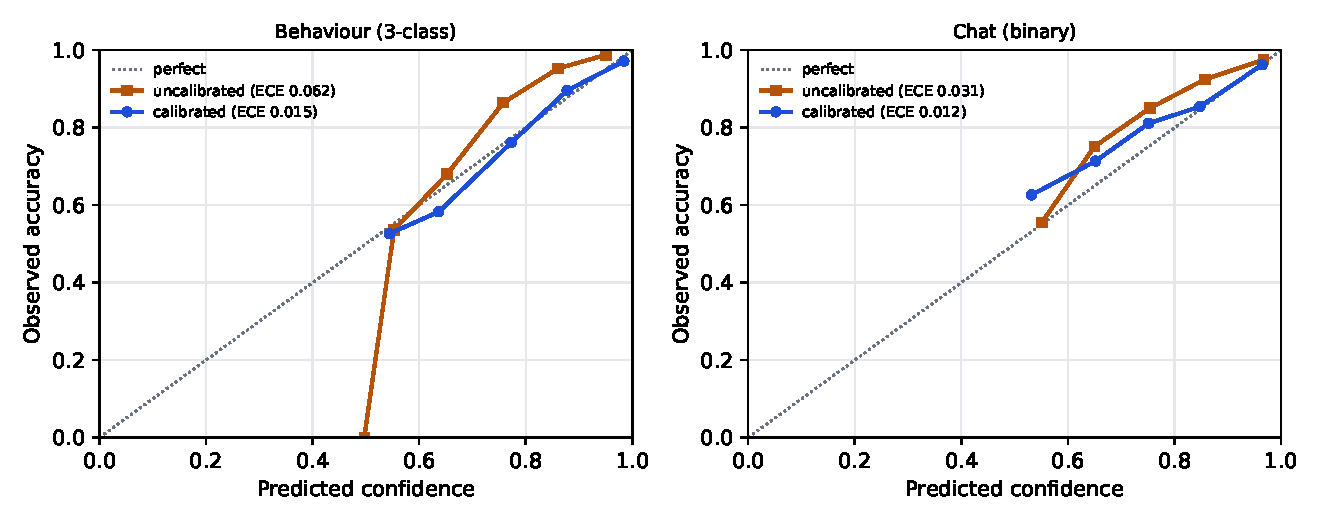
\includegraphics[width=\linewidth]{figures/reliability.pdf}
\caption{Reliability diagrams (top-label, 10 equal-width bins) for the two
calibrated channels, on the same held-out splits their isotonic layers were
fitted against. The diagonal is perfect calibration; ECE is the bin-weighted
mean gap between stated confidence and observed accuracy. Calibration cuts
behaviour ECE $0.062 \rightarrow 0.015$ (worst bin $0.50 \rightarrow 0.05$) and
chat ECE $0.031 \rightarrow 0.012$ --- the direct evidence behind every
``calibrated probability'' claim in this paper, which Brier alone (a mixture of
calibration and refinement) cannot provide.}
\label{fig:reliability}
\end{figure}

\begin{figure}[t]
\centering
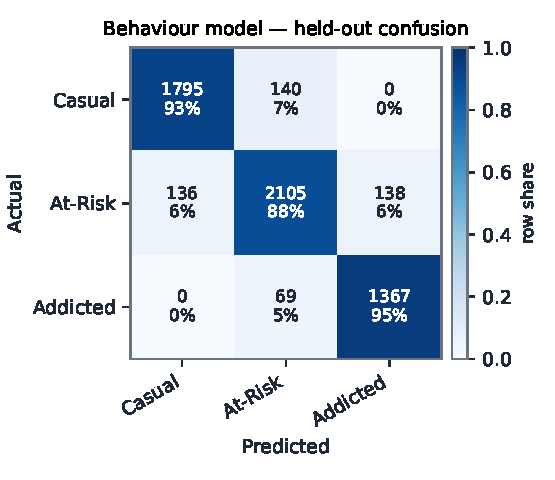
\includegraphics[width=0.5\linewidth]{figures/cm_behaviour.pdf}
\caption{Behaviour model, held-out confusion (counts and row share). Errors stay in
adjacent bands: both Casual$\leftrightarrow$Addicted corners are zero.}
\label{fig:cmbehaviour}
\end{figure}

\subsection{Chat toxicity model (gaming-domain trained; two evaluation views)}
\label{sec:chatresults}
Metrics are for the pipeline \emph{as served}: the isotonic-calibrated probability of
the word~$\cup$~char\_wb model trained on five real corpora (general toxicity +
CONDA train split + Davidson offensive-language tweets + HASOC 2019 Hindi in both
scripts + the clean-Hindi Wikipedia counterweight; held-out Brier $0.066 \rightarrow 0.063$,
top-label ECE $0.031 \rightarrow 0.012$ --- Fig.~\ref{fig:reliability}), fused
with the keyword lexicon. The held-out set is
reconstructed from the \emph{same} corpus assembly the trainer uses (shared code
path), so no training \emph{row} can re-enter it --- an earlier draft rebuilt this split
from the general corpus alone, which admitted trained CONDA/Davidson rows and
understated the realistic base rate. (Duplicate \emph{texts} are a subtler channel,
audited below.)
\begin{center}
\begin{tabular}{lccc}
\toprule
\textbf{Evaluation set} & \textbf{Precision (toxic)} & \textbf{Recall (toxic)} & \textbf{Note} \\
\midrule
Balanced held-out & 0.897 & 0.956 & optimistic view; PR-AUC 0.940 \\
General realistic stream @0.50 & 0.241 & 0.958 & 3.5\% toxic base rate \\
General realistic stream @0.95 (alert) & 0.433 & 0.398 & out-of-domain view \\
\bottomrule
\end{tabular}
\end{center}

\paragraph{Duplicate-text audit (net-conservative).} A provenance audit of the
assembled corpus found $18{,}038$ duplicate rows ($7.8\%$): the general corpus
itself carries a copy of the Davidson tweets alongside the canonical
\texttt{chat\_extra} file, and $6{,}542$ texts carried \emph{conflicting} labels
between their copies. Exact-duplicate texts therefore straddle the train/test
boundary ($10.6\%$ of balanced test rows had a training-side twin). Measured on
the pre-dedupe model, the net effect was \emph{conservative}, not inflationary:
the overlapping subset scored \emph{worse} than the rest (accuracy $0.840$ vs.\
$0.913$ overall), because a label conflict guarantees an error on one copy of the
text --- outweighing any memorisation gain --- so the leak-free subset read
accuracy $0.922$, PR-AUC $0.935$, Brier $0.062$, all slightly \emph{better} than
the then-published figures. That model was deliberately retained until the pilot
concluded (swapping models mid-pilot would confound the longitudinal score series
of \S\ref{sec:pilot}); the chat model was then retrained on the de-duplicated
assembly (one row per cleaned text, majority label, ties resolved toward toxic;
recorded by a metadata flag so evaluation always reproduces the exact assembly
the deployed model was trained on). The retrain confirmed the leakage analysis's
prediction: balanced held-out accuracy $0.913 \rightarrow 0.927$, PR-AUC
$0.926 \rightarrow 0.944$, Brier $0.070 \rightarrow 0.058$, while in-domain
\emph{ranking} is statistically unchanged (PR-AUC $0.833$ vs.\ $0.834$, inside
the bootstrap CI) --- and the alert threshold was re-derived from the new
calibrated curve per the standing procedure (below), moving from $0.90$ to
$0.95$. The subsequently adopted HASOC Hindi corpus (\S4.2, both scripts)
re-measured these figures once more (its Hindi rows make the balanced holdout
slightly harder --- accuracy $0.917$, Brier $0.066$ --- the price of a whole new
language in the corpus); the tables in this section report the final deployed
model.

\paragraph{In-domain evaluation on real gaming chat (held-out CONDA split).}
The serving domain is gaming chat, so the decisive evaluation is on \textbf{CONDA's
validation split} --- $7{,}721$ real Dota~2 utterances the retrained model
\emph{never saw}, toxic base rate $21.5\%$:
\begin{center}
\begin{tabular}{lccc}
\toprule
\textbf{Operating point} & \textbf{Precision (toxic)} & \textbf{Recall (toxic)} & \textbf{F1} \\
\midrule
@0.95 (deployed alert threshold) & \textbf{0.956} & 0.428 & 0.591 \\
@0.90 (recall-preferring option, env-selectable) & 0.888 & 0.623 & 0.732 \\
@0.85 (near best F1; selectable via env) & 0.800 & 0.703 & 0.749 \\
@0.97 (high-severity marker) & 1.000 & 0.024 & 0.046 \\
\bottomrule
\end{tabular}
\end{center}
The promised secondary views on this in-domain set: ROC-AUC $0.918$ and MCC $0.589$
at the alert threshold ($0.690$ at the $0.90$ point; per-configuration values for
every ablation row are in the released \texttt{ablation\_results.json} artifact).

\paragraph{Held-out Hindi evaluation --- both scripts (new capability, measured).}
Before the HASOC adoption the served pipeline caught \textbf{zero} Devanagari
abuse at the alert threshold (precision/recall $0.000$/$0.000$ on the held-out
Hindi set) and was nearly blind to \emph{romanised} Hindi abuse beyond the
keyword lexicon (PR-AUC $0.61$, recall $0.04$ at the alert point on the same
rows romanised). Three measured adoptions shaped the capability (the third ---
the clean-Hindi counterweight that drains a measured script-level toxicity
prior --- is described in \S4.2). First the
Devanagari rows (held-out PR-AUC $0.579 \rightarrow 0.875$); then, because the
bundled keyboard is QWERTY (typed Hinglish is \emph{romanised} in practice ---
\S5.2), each training row was added again in a colloquial romanisation
(ITRANS-based, via the \texttt{indic-transliteration}
library~\cite{indictrans}; the fetch script reproduces it deterministically). On the
$933$-row held-out split ($20\%$, stratified, never trained on; $52.9\%$
offensive base rate) the deployed model now reads, at the unchanged $0.95$
alert threshold: \textbf{Devanagari PR-AUC $0.890$, precision $0.968$ / recall
$0.425$; romanised PR-AUC $0.884$, precision $0.958$ / recall $0.366$} ---
$\geq$$0.95$ precision on \emph{every} register the system can capture
(English, Devanagari, romanised Hinglish), which is the uniform precision-first
guarantee the alert philosophy demands. The register recalls at the fixed
threshold are deliberately conservative; on the English in-domain set the
capability at \emph{matched} precision is unchanged through both adoptions
(CONDA PR-AUC $0.821$ after both Hindi adoptions vs.\ $0.833$ before them, inside
the bootstrap CI). Capture-path
honesty: the trained Devanagari path is fed by the accessibility capture
(system keyboards in non-canvas apps), the romanised path by the bundled
keyboard everywhere including canvas games, and spoken Hindi remains gated by
the Indian-English recogniser (\S5.2). \texttt{ml/eval\_chat\_hindi.py}
reproduces both views. A transformer reference completes the pattern here too: a
MuRIL-based Hindi abusive-speech model~\cite{das2022} ($\sim$236M parameters,
fine-tuned on aggregated Indic abusive corpora) reads PR-AUC $0.96$ on the
Devanagari view --- an upper bound, since overlap between its aggregated
training data and HASOC 2019 cannot be excluded (our fully-clean $0.890$ sits
closer than its size suggests) --- but $0.837$ on the
\emph{romanised} view, \emph{below} the deployed pipeline's $0.884$: on the
register the bundled keyboard actually carries, the deliberately
script-augmented classical model wins outright. The reading is consistent with
the chat and voice benchmarks (\S\ref{sec:modelselection},
\S\ref{sec:voiceresults}): capacity helps in-distribution; domain and register
fit decide.
Fig.~\ref{fig:prchat} shows the full precision--recall curve against the original
recipe: the deployed pipeline dominates at every operating point.
Three successive, measured improvements produced it, each adopted
only after a held-out comparison.

\begin{figure}[t]
\centering
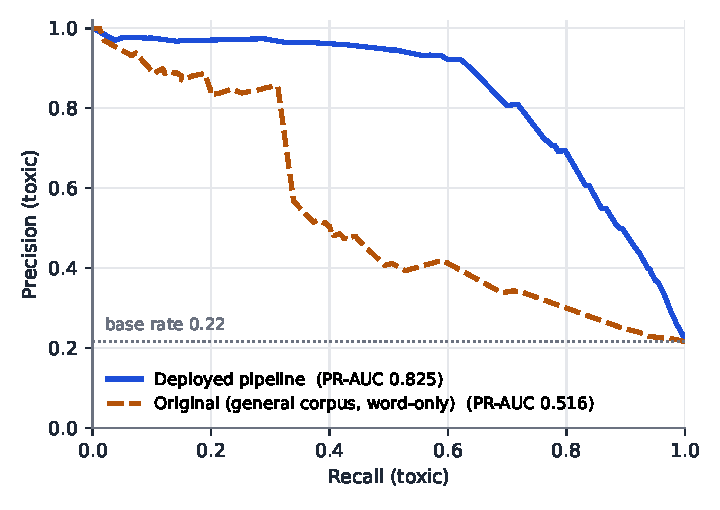
\includegraphics[width=0.68\linewidth]{figures/pr_chat.pdf}
\caption{Precision--recall on held-out real gaming chat (CONDA validation split,
$21.5\%$ toxic). The deployed pipeline (gaming-domain training, word$\cup$char\_wb
features, calibration, keyword fusion) dominates the original general-corpus recipe
across the entire curve.}
\label{fig:prchat}
\end{figure} Retraining on gaming-domain data lifted in-domain
PR-AUC from $0.549$ (general-corpus model) to $0.739$ --- confirming, with data, that
the earlier weak in-domain performance was a domain artifact. The
word~$\cup$~char\_wb feature union selected by the bake-off
(\S\ref{sec:modelselection}) lifted it to $0.805$, and adding the Davidson
offensive-language corpus (real informal/slang text) lifted it again to
$0.834$; the post-pilot de-duplicated retrain and the two Hindi adoptions
(audit and Hindi paragraphs above) hold at $\mathbf{0.821}$ served,
statistically unchanged through all three (every value in this chain lies inside
the others' bootstrap intervals; the $0.825$ in the ablation table of
\S
ef{sec:ablations} is the same recipe re-trained under that section's own
split and seed). Each revision \emph{re-derived the
alert threshold from its own held-out curve} --- calibration shifts where
probabilities land, so a threshold never survives a model change unexamined. On
the final model's calibrated scale the deployed $0.95$ threshold reads precision
$0.956$ at recall $0.428$ on English in-domain chat --- and \emph{every}
register clears $0.95$ precision at this one shared threshold (the same curve's
$0.90$ point reads $0.888/0.623$, available to a guardian who prefers recall ---
\texttt{CHAT\_ALERT\_T} is env-tunable), and the high-severity marker ($0.97$)
is right every time it fires (precision $1.00$ at recall $0.024$). The
pre-dedupe deployment's point read $0.950/0.491$ on its own scale, itself
strictly dominating its predecessors ($0.924/0.445$ before Davidson,
$0.891/0.266$ for the original general-corpus model). Per-message recall
deliberately traded away here is recovered at session level by the streak alert
below.

\paragraph{Session-level escalation recovers the remaining recall.}
Per-message alerting is deliberately precision-first, which caps per-message recall
--- but toxic players repeat, and repetition is itself evidence. The backend
therefore raises \emph{one aggregate ``repeated concerning language'' alert} when
three messages in a session score above a lower bar ($0.6$, where per-message recall
is $0.85$ in-domain at precision $0.60$), so repeated toxicity in a session
surfaces even when no single line crosses the per-message cutoff. The three
flagged messages are correlated (same speaker, same session), so the bar is a
repetition heuristic that suppresses one-off false positives, not an
independence-based probability bound.
General-corpus behaviour remains reported above for transparency: out-of-domain precision
is poor, which is expected --- and not directly representative of the serving
distribution, whose traffic is gaming chat.

\subsection{Voice emotion model (now trained on real audio)}
\label{sec:voiceresults}
The deployed voice model is trained on \emph{four real speech corpora}: RAVDESS
(1{,}440 clips, 24 speakers) $+$ CREMA-D (7{,}442 clips, 91 speakers of varied age
and ethnicity) $+$ EMO-DB (535 clips, 10 speakers, \emph{German}) $+$ URDU (400
clips, 29 speakers as distributed --- the release nominally lists 38, but 29
distinct speaker ids appear in the published files --- \emph{Urdu} --- included deliberately for its phonetic proximity
to the target users' Hindi). All $9{,}817$ clips are ingested \emph{through the
identical serving extractor} (silence floor $\rightarrow$ gain normalisation
$\rightarrow$ 36 features), with emotion labels mapped onto the system's four
classes, one noise/band-limit augmented variant per clip, and class balancing.
The classifier (\texttt{HistGradientBoosting}) and the extended feature set were
selected from a six-family bake-off under the speaker-independent protocol
(\S\ref{sec:modelselection}). On a \textbf{speaker-independent} held-out split
($31$ of $153$ speakers --- one of the $154$ ingested speakers contributed no clip
that survived the silence-floor gate --- $2{,}791$ rows; no test speaker appears in
training):
\begin{center}
\begin{tabular}{lcccc}
\toprule
\textbf{Metric} & \textbf{Angry} & \textbf{Excited} & \textbf{Frustrated} & \textbf{Neutral} \\
\midrule
F1 & 0.68 & 0.49 & 0.50 & 0.61 \\
\midrule
Accuracy & \multicolumn{4}{c}{\textbf{0.574}} \quad (chance $= 0.25$) \\
Macro-F1 & \multicolumn{4}{c}{0.568} \\
\bottomrule
\end{tabular}
\end{center}
This \emph{replaces} the earlier synthetic-feature model, whose $0.9925$ accuracy we
had already flagged as internal validity only. The protocol matters as much as the
number: under random clip splits this same configuration reads $0.657$, and the
$\approx 9$-point gap \emph{is the quantified speaker leakage} --- the model partly
recognising people rather than emotions (\S\ref{sec:evalmethod}). $0.574$ on unseen
speakers across three languages is the corrected generalisation number, and it is why
voice keeps its low, corroborating-only ensemble weight ($0.30$, tied with chat and
below behaviour's $0.40$). A transformer reference point was measured here too
(2026-08-04): the audEERING wav2vec2 \emph{dimensional} emotion
model~\cite{wagner2023} (trained on
natural, non-acted speech; arousal/valence outputs) scored zero-shot on the same
speaker-independent test clips under a common collapsed 3-class space
(negative-aroused / positive-aroused / neutral) reads $0.39$ vs.\ the deployed
model's $0.66$ --- with fixed quadrant thresholds it maps most negative-class
clips to neutral. The comparison cuts both ways (the transformer's home domain is
natural speech, the test set is acted corpora) and its lesson is narrower than
the chat channel's: an off-the-shelf dimensional model is \emph{not} a free
upgrade --- threshold calibration or fine-tuning would be required --- but its
natural-speech training remains the right starting point for the live domain gap
(Future Work names the deployable path).

\paragraph{Representation headroom (measured).} The $0.574$ is bounded by the
$36$ hand-crafted acoustic features, not by the classifier or the protocol. To
quantify that ceiling, frozen wav2vec2 embeddings ($1024$-d, from the same
audEERING model) were extracted for all $9{,}780$ clips and fed to the
\emph{identical} classifier family under the \emph{identical}
speaker-independent split (\texttt{ml/eval\_voice\_headroom.py}). The 36-feature
baseline reproduces at $0.553$ accuracy / $0.547$ macro-F1 (original clips, no
augmentation, so slightly below the augmented deployed number); the embedding
representation lifts it to $\mathbf{0.776}$ accuracy / $0.772$ macro-F1 ---
$+22$ points from representation alone, on unseen speakers. An honest negative
accompanies it: training on the corpora's \emph{fine} emotion labels and
grouping to the four served classes by summed probability \emph{underperformed}
the direct 4-class embedding model ($0.694$), because the fine classes are too
sparse per speaker under grouped splits. The reading for deployment: the
$512$\,MB serving budget is why embeddings are not served today, and it is
exactly why Future Work names the $72$K-parameter Wav2Small distillation --- this
experiment measures the prize ($\sim$$+20$ points) that distillation is chasing,
turning ``a bigger model would help'' from assertion into measurement.

That weight is \emph{nominal}: availability reweighting
raises voice's effective share when other channels are absent, and the pilot's
channel-contribution analysis (\S\ref{sec:pilot}) measures the real influence ---
removing voice would change roughly a third of served bands --- which is why the
channel's domain-shift mitigations are monitored, not assumed away. The earlier measured
gains survive the protocol correction in kind (variance features and corpus
diversity still help; the ablation table in \S\ref{sec:ablations} quantifies each
under the corrected protocol); the confusion structure
(Fig.~\ref{fig:cmvoice}) shows the expected excited$\leftrightarrow$frustrated
arousal confusions that the valence--arousal fusion with spoken words (\S5.3)
exists to resolve.

\begin{figure}[t]
\centering
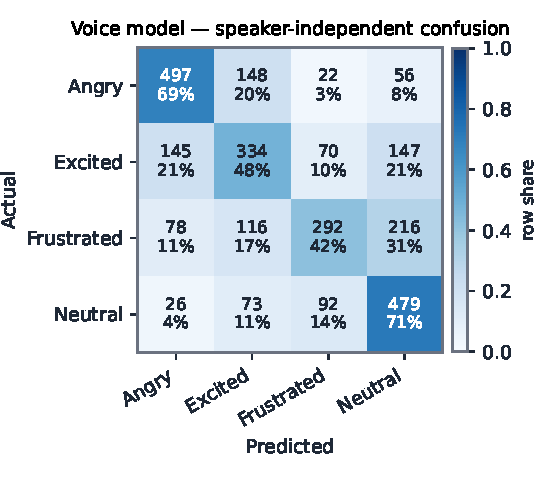
\includegraphics[width=0.5\linewidth]{figures/cm_voice.pdf}
\caption{Voice model, speaker-independent held-out confusion. Errors concentrate in
the arousal-sharing pairs (excited$\leftrightarrow$angry,
frustrated$\rightarrow$neutral) that the word-level valence fusion targets.}
\label{fig:cmvoice}
\end{figure} The confusions are the expected ones
(excited$\leftrightarrow$frustrated share high arousal; the valence--arousal fusion
with the spoken words, \S5.3, exists precisely to resolve them). The remaining
caveat, stated plainly: all four speech corpora are \emph{acted, adult} speech --- closer to
reality than synthetic features but still not child gaming speech, which stays the
validation target.

\subsection{ASR accent-fairness audit (spoken-chat front end)}
\label{sec:asrfairness}
The spoken-chat path chains the on-device Indian-English recogniser into the
served toxicity scorer, and \S7 argues that such a chain owes its users a
fairness audit: a transcription error that \emph{creates} a toxic word would
concentrate false accusations on whoever the acoustic model serves worst. We
executed the accent axis of that audit on Svarah~\cite{svarah2023} --- $6{,}656$
clips / $9.6$ hours of transcribed Indian-English from $117$ speakers across
$65$ districts, each carrying the speaker's primary language --- by
transcribing every clip with the \emph{deployed} recogniser
(\texttt{vosk-model-small-en-in-0.4}) and pushing every hypothesis through the
\emph{served} scoring formula (clean $\rightarrow$ TF-IDF $\rightarrow$
calibrated LogReg, noisy-OR keyword fusion, alert at $0.95$).
Reproduction: \texttt{ml/eval\_asr\_fairness.py}; aggregate output ships as
\texttt{docs/asr\_fairness.json}.

\textbf{Finding 1 --- the alert path is accent-safe at the deployed threshold.}
Across all $6{,}656$ benign clips the chain raised \textbf{zero} false toxicity
alerts --- on the ASR hypotheses \emph{and} on the human reference transcripts
(the no-ASR control). Zero observed events bound the benign-speech alert FPR at
$\leq 0.045\%$ overall (rule of three, $95\%$), and $\leq 0.75\%$ even for the
smallest per-family stratum. Despite a $38.6\%$ overall word-error rate ---
plenty of raw material for hallucinated profanity --- the precision-first
threshold plus domain-trained scorer never converted a mis-transcription into
an accusation. The equity failure mode \S7 warns about is, at this threshold
and on this benchmark, not observed in any group.

\textbf{Finding 2 --- but recognition quality is not accent-uniform, so
\emph{coverage} is.} WER stratifies cleanly by language family: Dravidian-L1
speakers $34.6\%$ ($n{=}1{,}798$ clips), Indo-Aryan $38.1\%$ ($n{=}4{,}456$) ---
and Tibeto-Burman $60.8\%$ ($n{=}402$), $1.76\times$ the Dravidian rate.
Per-language extremes run Tamil $30.9\%$ to Bodo $60.8\%$, essentially
$2\times$, with the Northeast (Bodo, Assamese $51.4\%$, Nepali $42.8\%$)
occupying the entire worst tail. Gender, by contrast, is balanced ($38.4\%$
female vs $38.7\%$ male). The fairness impact is therefore \emph{asymmetric}:
no group is falsely accused, but for Northeast-Indian speakers the recogniser
recovers barely two words in five, so genuinely toxic speech is
correspondingly less likely to be \emph{caught} --- a recall gap, not a
false-positive gap, concentrated on under-served accents. The honest summary
for the model card is ``the voice-to-chat channel hears some Indian accents
markedly worse than others, and degrades toward silence, not toward false
alarms.''

\textbf{Scope, stated plainly.} Svarah is adult read and conversational
speech, so this audit bounds the \emph{accent} axis only; the gaming-domain
axis is exercised separately by the spoken-chat smoke tests
(\S\ref{sec:chatresults}), and \emph{toxic} accented speech --- needed to turn
the recall-gap inference into a measured per-accent recall --- exists in no
open corpus we could locate. The absolute WER also reflects a deliberate
trade: a $50$\,MB on-device model keeps raw audio off the network entirely,
at an accuracy cost server-scale ASR would not pay. The actionable output is
specific: Northeast-accent adaptation data is the highest-leverage STT
improvement the system could adopt, and any future recogniser swap
(\S\ref{sec:futurework}) should be gated on re-running this audit, which is
now a two-command reproducible artefact.

\subsection{Ablation studies}
\label{sec:ablations}
One component is removed per row from the deployed recipe and re-measured on the
same fixed held-out data, so each delta is attributable; brackets are bootstrap
$95\%$ CIs (\S\ref{sec:evalmethod}).

\textbf{Chat} (held-out CONDA validation split; PR-AUC primary):
\begin{center}
\begin{tabular}{lcc}
\toprule
\textbf{Configuration} & \textbf{PR-AUC [95\% CI]} & \textbf{Precision@0.95} \\
\midrule
Full recipe (deployed)            & 0.825 [0.807, 0.841] & 0.965 \\
$-$ keyword-lexicon fusion        & 0.814 [0.796, 0.830] & 0.973 \\
$-$ calibration                   & 0.837 [0.820, 0.852] & 0.965 \\
$-$ char\_wb n-grams              & 0.794 [0.777, 0.811] & 0.963 \\
$-$ Davidson corpus               & 0.794 [0.775, 0.812] & 0.895 \\
$-$ HASOC Hindi corpus (both scripts) & 0.832 [0.815, 0.848] & 0.958 \\
$-$ clean-Hindi wiki counterweight & 0.835 [0.818, 0.850] & 0.964 \\
$-$ CONDA corpus (domain data)    & 0.511 [0.487, 0.535] & 0.906 \\
Original (general-only, word-only) & 0.516 [0.490, 0.539] & 0.889 \\
\bottomrule
\end{tabular}
\end{center}
Domain data dominates everything else combined ($+0.31$ PR-AUC) --- removing CONDA
collapses the model below even the original recipe's curve shape. Character n-grams
($+0.030$) and Davidson ($+0.031$) are
each significant. The two Hindi rows are deliberately read differently: their
CONDA deltas are small and \emph{negative} ($-0.007$ and $-0.010$, inside the
CIs) --- a Hindi corpus cannot improve an English-chat metric, and the honest
reading is that the multilingual capability costs a within-noise sliver of
English ranking --- while their measured contribution lives entirely in the
held-out Hindi evaluation above ($\geq$$0.95$ alert precision on both scripts
from near-zero, and the drained script prior), which is
why corpus adoptions are judged on capability, not on a single aggregate score.
Two nuances: the keyword fusion buys only $+0.011$ PR-AUC --- and a telling
second-order effect: with the romanised-Hindi rows trained in, the lexicon's
alert-recall contribution shrank from $+0.05$ to under $+0.01$, because the
trained model now carries most of what the hand-curated lexicon alone once
provided; the lexicon is retained for interpretability and same-day coverage of
novel slang, not ranking. And
\textbf{calibration costs $0.012$ PR-AUC}: isotonic regression creates probability
plateaus (ties) that coarsen ranking. We accept that deliberately --- on the
calibrated scale the $0.95$ threshold \emph{empirically achieved} $96\%$ held-out
in-domain precision (the served score is the calibrated probability fused with the
lexicon by noisy-OR, so the guarantee is the measured operating point, not
calibration theory), and threshold
semantics matter more to this product than the last centile of ranking resolution.

\textbf{Voice} (speaker-independent; fixed test set of $1{,}880$ original clips from
$31$ unseen speakers; training side varies):
\begin{center}
\begin{tabular}{lcc}
\toprule
\textbf{Configuration} & \textbf{Accuracy [95\% CI]} & \textbf{Macro-F1} \\
\midrule
Full (36 features, 4 corpora, aug$\times$1) & 0.562 [0.540, 0.584] & 0.557 \\
17-feature prefix                           & 0.499 [0.476, 0.521] & 0.488 \\
$-$ augmentation                            & 0.566 [0.545, 0.589] & 0.561 \\
English-only training corpora               & 0.546 [0.525, 0.568] & 0.541 \\
\bottomrule
\end{tabular}
\end{center}
The 36-feature extension is the one \emph{significant} factor ($+6.3$ points,
disjoint CIs) --- the MFCC-variance and spectral cues carry real signal. The
noise/band-limit augmentation is measurably \emph{neutral} on studio corpora (its
robustness rationale targets real phone-mic conditions, which only the pilot can
test); multilingual training data adds a small positive on the multilingual test
($+1.7$, overlapping CIs) and is required regardless for the Urdu/Hindi target
population. (Deployed-model numbers in \S\ref{sec:voiceresults} differ slightly
because the trainer's test side also contains augmented variants; the ablation table
tests original clips only.)

\textbf{Behaviour} (synthetic, survey-grounded generator):
\begin{center}
\begin{tabular}{lcccc}
\toprule
\textbf{Feature set} & \textbf{Accuracy [95\% CI]} & \textbf{Macro-F1} & \textbf{QWK} & \textbf{Non-adj.} \\
\midrule
Screen-time only (hours --- the baseline) & 0.702 [0.690, 0.714] & 0.709 & 0.757 & 7 \\
Objective-10 (deployed)          & 0.916 [0.909, 0.923] & 0.918 & 0.928 & 0 \\
All-20 (incl.\ derived proxies)  & 0.919 [0.912, 0.926] & 0.921 & 0.931 & 0 \\
Volume features only (5)         & 0.871 [0.861, 0.879] & 0.874 & 0.890 & 0 \\
Pattern features only (5)        & 0.902 [0.894, 0.910] & 0.905 & 0.916 & 0 \\
\bottomrule
\end{tabular}
\end{center}
Because Casual $<$ At-Risk $<$ Addicted is an \emph{ordered} scale, the table also
reports quadratic-weighted kappa (QWK --- errors penalised by squared band
distance) and the count of \emph{non-adjacent} errors (two-band jumps,
Casual$\leftrightarrow$Addicted), which plain accuracy and F1 price no differently
from a one-band miss. The first row is the \emph{thesis baseline}: the project's
core claim is that rich behavioural patterns beat screen-time counting, so the
table must contain screen-time counting. Deliberately given its best shot --- both
hours features, the same model family, protocol and CIs as every other row --- a
well-fit hours-only model reaches $0.702$, \textbf{21.4 points below the deployed
feature set} with cleanly disjoint intervals; and the ordinal view sharpens the
verdict --- the hours-only model commits \textbf{seven} Casual$\leftrightarrow$Addicted
two-band errors on the 5{,}750-row test set, a failure mode \emph{every} richer
feature set avoids entirely. The central claim is measured, not asserted. The derived
proxies add nothing beyond the objective ten (overlapping CIs --- confirming
\S\ref{sec:features} empirically). More interesting: the five \emph{pattern}
features (late-night ratio, streak, binges, breaks, rapid re-logins) alone recover
$0.902$, while the five \emph{volume} features (hours, sessions, duration) reach
only $0.871$ --- the model leans on \emph{how} a child plays more than on \emph{how
much}, which is precisely the DSM-5/ICD-11 framing that motivated the feature
design. (Caveat, stated once for the whole table: these rows share the
survey-grounded synthetic generator, so they measure the information structure of
the feature space, not clinical validity --- the IGDS9-SF study
(\S\ref{sec:survey}) is the external anchor. On the pattern-versus-volume row
specifically, that anchor now agrees: against \emph{real} IGDS9-SF severity in
$103$ respondents, the pattern composite reaches $\rho = 0.330$ and the volume
composite only $0.128$ with a CI including zero --- the same ordering, obtained
without the generator that could have manufactured it.)

\subsection{ML pipeline revisions: what changed, why, and the measured effect}
\label{sec:mlrevisions}
This iteration revised the ML pipeline in six ways. Each row states the motivation
and the measured (not asserted) consequence. Figures are \emph{as measured at that
revision}; where a later revision re-measured the same quantity, the final number in
the Results sections supersedes it --- notably the chat calibration row's held-out
Brier ($0.088 \rightarrow 0.075$ then) predates the eval-leakage correction of
\S\ref{sec:chatresults}, whose final held-out Brier (post-dedupe retrain with the
dual-script HASOC Hindi corpus and the clean-Hindi counterweight) is
$0.066 \rightarrow 0.063$.

\begin{xltabular}{\linewidth}{p{3.1cm}XX}
\caption{ML pipeline revisions: motivation and measured effect of each change.}
\label{tab:revisions}\\
\toprule
\textbf{Change} & \textbf{Why} & \textbf{Measured effect} \\
\midrule
\endfirsthead
\multicolumn{3}{@{}l}{\footnotesize\tablename~\thetable\ --- \emph{continued}}\\
\toprule
\textbf{Change} & \textbf{Why} & \textbf{Measured effect} \\
\midrule
\endhead
\bottomrule
\endlastfoot
Behaviour model input reduced to the ten objective features &
The ten psychometric proxies are deterministic functions of the objective ten ---
zero added information, and SHAP could present a derived score to a parent as if
independently measured (circular explanation) &
Held-out accuracy unchanged ($92.3\%$ vs.\ $92.4\%$), confirming the redundancy;
every served SHAP factor now cites a genuinely measured behaviour \\
\addlinespace
Isotonic calibration layer on the chat model &
The behaviour channel was calibrated but chat was not; an uncalibrated probability
makes any fixed alert threshold arbitrary &
Held-out Brier $0.088 \rightarrow 0.075$; alert threshold re-chosen on the calibrated
scale from the measured realistic curve ($0.85$), raising realistic alert precision
$0.074 \rightarrow 0.088$ \\
\addlinespace
Noisy-OR fusion of lexicon + model toxicity (was \texttt{max()}) &
\texttt{max()} discards the weaker of two \emph{independent} evidence sources; two
moderate signals are jointly stronger than either alone &
Output remains probability-shaped and $\geq$ \texttt{max()} by construction;
confidently toxic test messages score higher (e.g.\ $0.98$) while clean gaming chat
stays low ($\approx 0.17$) \\
\addlinespace
Voice-activity detection gate (\texttt{webrtcvad}) + shared extraction module &
An energy floor cannot reject \emph{game audio/music}, the dominant real contaminant;
extraction previously lived only in the backend, risking future train/serve skew &
Non-speech segments degrade to low-confidence neutral instead of spurious emotions;
one extractor now provably feeds both serving and training \\
\addlinespace
Env-tunable thresholds + Beta-posterior feedback tuner &
Threshold changes required a code deploy; parent verdicts (the only real labels) had
no mechanism to influence the system &
Verified on synthetic verdicts: $6/8$ false alarms in the Addicted band recommends
$+0.038$ on that cut-point; sparse bands are left untouched \\
\addlinespace
PR-AUC + Brier reporting; in-domain chat evaluation; real-audio voice retraining;
reflections correlation analysis &
Single-threshold rows hide the operating curve; domain transfer was asserted, not
tested; voice was the only synthetically-trained channel; the daily check-ins were
unused as an outcome signal &
Model card carries threshold-free metrics; voice model \emph{retrained} on real
speech (RAVDESS+CREMA-D, 115 speakers): $0.572$ accuracy --- then still measured
under random clip splits; the speaker-independent correction lands two rows below
--- replaces the $0.9925$
synthetic figure (\S\ref{sec:voiceresults}); risk-vs-next-day-mood correlation
computable from data already collected \\
\addlinespace
Chat model retrained on gaming-domain data; alert threshold re-chosen (then
$0.95$/$0.97$, later recalibrated to $0.90$/$0.95$ on that model's scale; the
post-dedupe retrain re-derived the pair again, to the current $0.95$/$0.97$ ---
\S\ref{sec:chatresults}); session-level streak alert &
General-corpus training was the measured root cause of weak in-domain performance;
per-message precision-first alerting caps recall, but toxic players repeat &
Held-out gaming PR-AUC $0.549 \rightarrow 0.739$; repeated moderately-flagged messages now
raise one aggregate alert (per-message recall $0.92$ at the streak bar) \\
\addlinespace
Model-family bake-offs for all three channels; chat gains char\_wb n-grams; voice
gains MFCC-variance + spectral features and \texttt{HistGradientBoosting} &
Model choices rested on convention; each deserved a measured comparison matched to
what its data can support &
Behaviour: five families within $0.6$\,pp on CV (even the linear baseline) $\rightarrow$
RandomForest retained for SHAP/calibration, now by evidence; chat: held-out gaming
PR-AUC $0.739 \rightarrow 0.805$, alert precision $0.924$; voice: six families
compared, \texttt{HistGradientBoosting} adopted on speaker-independent evaluation
(RBF-SVM led on random splits but the edge was speaker leakage; see
\S\ref{sec:modelselection}), speaker-independent accuracy $0.574$ \\
\addlinespace
Behaviour play-time distributions + peer-percentile table grounded in a real survey
of $13{,}464$ gamers (Sauter \& Draschkow 2017, CC-BY) &
The generator's play-time bands and the dashboard's peer percentiles were invented;
the peer table was measurably wrong (10\,h/wk shown as 45th pct; real: 20th) &
Casual/at-risk/heavy weekly hours now follow empirical percentile segments of the
aged-$\leq$24 cohort ($n{=}11{,}731$); accuracy moves $0.923 \rightarrow 0.916$
because \emph{real} class overlap is larger --- the more realistic number; direction
check: hours vs.\ anxiety $r{=}{+}0.065$, vs.\ life satisfaction $r{=}{-}0.119$ \\
\addlinespace
Corpus expansion: chat gains Davidson offensive-language tweets ($24{,}783$ real);
voice gains EMO-DB (German) + URDU, reaching $154$ speakers / 3 languages &
More real data in the registers that matter --- informal slang-heavy text for chat;
speaker, age and language diversity (Urdu $\approx$ target users' Hindi) for voice &
Chat held-out gaming PR-AUC $0.805 \rightarrow 0.834$; new alert point
\emph{strictly dominates} ($0.950$/$0.491$ vs.\ $0.924$/$0.445$); voice real-speech
accuracy $0.645 \rightarrow 0.657$ on a larger, more diverse held-out set
(random-split era; superseded by the speaker-independent protocol in the final row) \\
\addlinespace
Fusion/usage audit: session chat score $\rightarrow$ max of per-message scores;
anomaly detector $\rightarrow$ robust median/MAD $z$; ensemble weights, genre
multiplier, voice-risk mapping and valence--arousal weights audited and
\emph{deliberately left as documented priors} &
The concatenated-blob session score diluted a lone toxic line and disagreed with the
alert path; std-based $z$ lets one past binge day mask the next; the priors have no
labels to fit and fitting them on synthetic data would be circular &
Max aggregation wins on 707 real conversations (PR-AUC $0.916$ vs.\ $0.907$) and
removes TF-IDF from the hot path; outlier-masking fix is unit-tested; the prior
components remain env-/feedback-tunable rather than silently ``optimised'' \\
\addlinespace
Evaluation methodology hardened: speaker-independent voice splits; ablation studies
with bootstrap CIs; PR curves + confusion-matrix figures; PR-AUC/ROC-AUC/MCC/Brier
metric suite &
Random clip splits leak speaker identity; single-threshold rows and headline
accuracies hide error structure, uncertainty and the contribution of each design
choice &
Leakage quantified ($0.657 \rightarrow 0.574$, and it had been selecting the wrong
model); every design choice now carries a measured, CI-qualified delta
(\S\ref{sec:ablations}); domain data revealed as the dominant chat factor
($+0.32$ PR-AUC) \\
\end{xltabular}

The unifying principle is the paper's existing stance --- honesty over headline
numbers: remove information the model only \emph{appears} to use, calibrate what is
served, choose thresholds from measured curves, gate inputs the model was never
trained to see, and build the instruments that let real labels --- not synthetic
assumptions --- drive the next revision.

\subsection{System and engineering results}
\begin{itemize}[leftmargin=1.4em]
  \item Production-deployed cloud backend (HTTPS, token auth, consent, durable
        managed Postgres); both apps build as signed release APKs.
  \item A layered test program, all passing: a 180-test API suite (isolated database;
        includes ML-unit tests for the shared audio extractor, noisy-OR fusion,
        threshold-tuner math and the session-streak alert; run automatically in CI
        against \textbf{both} SQLite and PostgreSQL~16 --- the production dialect ---
        on every push), an \textbf{82-check functional sweep run in production auth mode} with real
        parent/child tokens (registration and family joins, role guards on every
        parent-only endpoint, the full nudge lifecycle, a real WAV upload through the
        silence floor and late re-score, the watchdog's quiet hours, end-session
        idempotency, feedback re-rating, parent-controlled deletion), and a
        \textbf{25-check end-to-end probe of the live cloud deployment}. A fifth layer
        generates cases nobody wrote: \textbf{property-based API fuzzing}
        (Schemathesis~\cite{schemathesis}) over all 53 documented operations, plus a
        dependency-CVE audit (\texttt{pip-audit}). Under the production auth posture the
        fuzz produced \textbf{no server errors}; it did find one real precedence
        bug --- an endpoint that parsed its JSON body \emph{before} authenticating, so
        an unauthenticated caller received \texttt{415} (``this endpoint wants JSON'')
        instead of \texttt{401} --- now fixed, regression-tested, and confirmed by a
        scripted scan to have been the only such endpoint
        (\texttt{docs/API\_FUZZ\_REPORT.md}). The same pass retired six dependency
        CVEs (\texttt{pip-audit}), added Python static security analysis to match the
        apps' MobSF scan (\texttt{bandit}~\cite{bandit}: 44 medium findings, \emph{43 verified false
        positives} --- a script proved every flagged SQL string interpolates only a
        dialect placeholder or a hardcoded identifier, never user input --- and one
        real \texttt{eval} in test code, replaced with \texttt{ast.literal\_eval}), and
        confirmed by a committed-secret scan (\texttt{detect-secrets}~\cite{detectsecrets}) that no service-account
        key, signing keystore or server secret is tracked in this \emph{public}
        repository or ever was. Statement coverage of the suite is $75\%$ overall
        ($80\%$ excluding developer-only utility scripts). Both apps pass
        Android Lint with zero errors, and 110 JVM unit tests (run in CI) pin offline
        session/capture-health transitions, profile and risk-presentation rules, the
        offline chat queue's delivery semantics, the WAV container encoding, IME
        keystroke-to-sentence reconstruction, and parent-alert triage.
  \item Robustness under load on free-tier hosting: pooled, probe-validated connections
        to the serverless Postgres (replacing per-request TLS handshakes; connections
        killed by scale-to-zero are detected and replaced transparently), per-client
        rate limiting behind the reverse proxy (previously all users shared one
        per-proxy quota --- the cause of earlier failures under load), memoised SHAP
        explanations and a throttled anomaly scan on the 30-second polling path, a
        16\,MB request-body cap, and threaded single-worker serving sized to the
        512\,MB instance. Verified with a concurrent smoke test (288 mixed requests
        across 24 threads, zero errors; re-verified after the heavier chat vectorizer
        landed --- p50 80\,ms, p95 609\,ms --- via the permanent
        \texttt{scripts/concurrency\_smoke.py}). On the device side, state shared across the
        monitor, accessibility, keyboard and notification threads is made thread-safe
        (concurrent game-detection cache; a crash-safe offline chat queue that removes a
        line from disk only after the server confirms it, so a process death mid-flush
        loses nothing), and background push declares a default
        notification channel so a high-risk alert to a backgrounded parent is delivered
        at full priority.
  \item Graceful degradation when a modality is absent; an idempotent session-end (a
        repeated end --- manual plus the passive auto-end, or a retry --- returns the
        existing result, with its full per-model sub-scores, instead of double-counting);
        a self-healing stale-session guard that also \emph{scores and raises the parent's
        risk alert} for the sessions it closes (from the snapshots captured live, so a
        lost end-event still appears in the risk history --- and a high-risk one still
        alerts the parent --- rather than vanishing silently); and an on-device offline
        retry queue for chat captured without connectivity (kept on a server or transient
        429/408 error, so nothing is silently dropped).
\end{itemize}

\subsection{Real-device validation (and what it caught)}
Beyond the automated layers, the complete system was exercised on a physical Android~16
handset against the live cloud deployment: registration $\rightarrow$ consent
$\rightarrow$ the guided permission chain $\rightarrow$ \emph{automatic} session
detection on a real game (Roblox, no manual start) $\rightarrow$ live microphone
capture with on-device Vosk transcription (voice events and speech-to-text lines
arriving server-side and feeding the fusion) $\rightarrow$ automatic session end with a
scored prediction $\rightarrow$ the parent-side flows. This pass surfaced three
production-class defects that no amount of local or API-level testing had caught ---
each was fixed and is now regression-guarded:
\begin{enumerate}[leftmargin=1.4em]
  \item \textbf{Launch crash on modern Android.} Reading the enabled-keyboards system
        setting throws a \texttt{SecurityException} for apps targeting SDK~$>$~33, so
        the permission-chain check crashed the Home screen on Android~12+ devices; the
        check now uses the supported \texttt{InputMethodManager} API, and the
        remaining system-settings reads are wrapped to degrade to a re-prompt rather
        than a crash.
  \item \textbf{Out-of-memory under live voice load.} Real gameplay streams a voice
        segment every $\sim$10 seconds; several analysed concurrently pushed the
        512\,MB instance over its limit and triggered a platform restart. Fixed by the
        audio-analysis semaphore, burst-collapsing the per-segment re-score, more
        frequent worker recycling, and single-threaded BLAS (\S3.2).
  \item \textbf{A notification feedback loop.} The Parent dashboard (which shows the
        \emph{day roll-up} band) and the alert poller (which compares the
        \emph{latest-session} band) both wrote the same ``last seen risk'' state; near
        a band boundary the two disagreed, so every poll saw a ``change'' and re-fired
        the risk-change notification indefinitely. The band-comparison notification
        was ultimately removed outright: notifications now derive solely from durable
        alert rows, deduplicated by alert id, so there is no shared band state left
        to flap.
\end{enumerate}
We report these candidly: they are precisely the class of defect that only
real-device, real-network operation reveals, and finding and fixing them --- rather
than not looking --- is part of the production-readiness this paper claims.

\subsection{Live family pilot: first real-world results}
\label{sec:pilot}
A consented family pilot began on 6~July~2026: release APKs sideloaded onto family
devices, talking to the production cloud deployment. Instrumented data collection
spans 6--28~July (23 days); a consent-version rollout then required a re-consent
that was never completed on the pilot device, so ingestion ceased \emph{fail-closed}
--- the consent architecture operating exactly as designed --- and enrolment
formally concluded in early August 2026. Over the first 12 days the system
recorded, unattended, \textbf{55 auto-detected sessions} across 11 active days
($\sim$7 hours of play, dominated by a casual title with no in-game chat),
\textbf{1{,}660 served predictions}, 1{,}211 chat-channel rows, 1{,}759 voice events,
1{,}675 screen events, and \textbf{60 alerts spanning all eight alert types}, of which
the parent read 52 --- real engagement, not a dormant install. Table~\ref{tab:pilot}
summarises the collected corpus.

\begin{table}[ht]
\centering
\footnotesize
\caption{Pilot data collected in the first 12 days (6--18 July 2026), by channel.
Chat/toxicity alerts reflect the then-deployed $0.90$ alert threshold; the
post-pilot retrain re-derived it to $0.95$ (\S\ref{sec:chatresults}).}
\label{tab:pilot}
\begin{tabularx}{\linewidth}{@{}lrX@{}}
\toprule
\textbf{Stream} & \textbf{Rows} & \textbf{Composition / quality notes} \\
\midrule
Sessions & 55 & 11 active days, 2 children; all auto-detected; avg 7.5\,min;
zero stuck-open, zero unscored \\
Predictions & 1{,}660 & presence: voice 99.9\%, behaviour 3.7\%, chat 0.4\%;
bands 51\% casual / 49\% at-risk \\
Chat rows & 1{,}211 & 1{,}209 via on-device STT, 2 typed (keyboard IME was reset
mid-pilot, see below); 2 crossed the 0.90 alert bar \\
Voice events & 1{,}759 & durations 5--10\,s post-VAD; intensity spread 0.20--1.00;
\textbf{0 rows retain audio}; label skew: 77\% frustrated in this 12-day window (see below) \\
Screen events & 1{,}675 & 652 on / 667 off / 356 unlock (balanced on/off = no
receiver gaps); 208 late-night --- live sleep-signal data \\
Alerts & 60 & all 8 types exercised (risk, toxicity, streak, offline, permission,
tamper, login, session); 52 read by the parent \\
Parent verdicts & 17 & first real labels; drive the threshold tuner (\S5.6) \\
\bottomrule
\end{tabularx}
\end{table}

The pilot's findings, positive and negative alike:
\begin{itemize}[leftmargin=1.4em]
  \item \textbf{Session lifecycle: zero defects.} No session was left stuck open and
        none went unscored --- automatic detection, grace-period ending and
        stale-session healing ran for 12 days without manual intervention.
  \item \textbf{The full spoken-abuse chain fired in production.} Two on-device
        transcripts crossed the $0.90$ alert threshold; the resulting toxicity and
        toxicity-streak alerts were delivered to and read by the parent. The paper's
        headline pipeline --- on-device STT $\rightarrow$ calibrated toxicity fusion
        $\rightarrow$ precision-first alert --- has now operated end-to-end on real
        speech, unprompted.
  \item \textbf{Privacy guarantees held under load:} of 1{,}759 voice events, exactly
        \textbf{zero} retained an audio file --- the raw-audio-deletion policy verified
        in production, not just in tests.
  \item \textbf{Availability-weighted fusion proved necessary, not hypothetical.}
        Real modality presence was voice $99.9\%$, behaviour $3.7\%$, chat $0.4\%$ of
        live re-scores: channels genuinely appear and vanish per game and moment,
        which is exactly the condition the renormalising ensemble (\S3.2) was designed
        for.
  \item \textbf{Tamper/permission monitoring caught two real events.} On one device
        the custom keyboard was silently disabled mid-pilot (an OS default-IME reset):
        the heartbeat's capture-permission flags flipped, the parent dashboard showed
        ``monitoring degraded'', and a one-shot alert fired. On the second device, the
        anti-tamper design met an actual tamper: a participant deactivated Device
        Administrator and uninstalled the app --- \texttt{onDisableRequested} raised
        the high-severity ``trying to remove monitoring'' alert \emph{four seconds
        before the device went silent for good}. The uninstall was detected in real
        time, exactly as designed; the removal itself was, of course, the
        participant's right.
  \item \textbf{The fusion-prior audit exposed sensitivity, a unit-of-analysis
        limitation --- and, once corrected, a changed conclusion.} An initial
        exploratory run over 1{,}961 served snapshots suggested weight perturbations
        changed at most $0.3\%$ of bands. An internal review of the analysis script found that long sessions
        contributed many correlated live re-scores and floating-point boundary
        comparisons omitted 14 of the intended 37 weight combinations; the corrected
        \texttt{ml/analyze\_fusion\_sensitivity.py} uses exactly the latest
        prediction from each completed session, preserves the observation-mode
        ceiling, covers all 37 grid points, and refuses output unless it reproduces
        every served score and category. Rerun on the production pilot database
        (131 completed pilot sessions, demo/probe accounts excluded; replication
        max $|\Delta| = 6{\times}10^{-5}$), the
        corrected picture is \emph{less} flattering than the exploratory one --- which
        is exactly why the rerun mattered: weight perturbations of $\pm 0.15$ flip a
        median $0.8\%$ and worst-case $10.7\%$ of session bands (not $0.3\%$),
        removing the genre multiplier flips $34.4\%$, and $\pm 0.05$ threshold
        shifts flip up to $26.7\%$. The stakes ranking stands --- thresholds and the
        genre effect are the high-stakes priors, the weights moderate --- and is
        precisely why the IGDS9-SF study targeted both first. It has since
        returned a verdict on each, and neither changed the deployment:
        the fitted thresholds are declined because the sample's missing severity
        tail is what pins them, and the genre multiplier is retained-but-flagged
        because its null is underpowered rather than decisive
        (\S\ref{sec:survey}). A
        prevalence-anchoring method for the top-band threshold is implemented and
        population-gated (\texttt{ml/calibrate\_thresholds\_prevalence.py}).
  \item \textbf{Channel contribution to the fused decision, measured on real
        traffic.} The same replication-gated analysis re-fuses each session using
        only a subset of its captured channels (weights renormalised, genre and
        observation-cap policy unchanged --- exactly what serving would have
        produced had the other channels never been captured). On the pilot's 131
        sessions: behaviour alone agrees with the full decision in only $67.7\%$ of
        sessions --- i.e.\ \emph{removing voice changes the parent-visible band
        roughly a third of the time} --- while dropping behaviour (chat+voice only)
        flips $12.5\%$. Behaviour+voice reproduces the served decision exactly
        ($100\%$, mean $|\Delta\text{score}| < 10^{-3}$) because typed chat was
        structurally absent in this pilot's no-chat title --- the
        availability-weighted design operating as intended. Two readings
        follow: the multimodal fusion demonstrably changes decisions on real data
        (it is not behaviour with decoration), and voice's substantial influence is
        exactly why its documented domain-shift bias (\S6.3) and lowest prior
        weight matter --- a channel this influential must earn its labels, which is
        what the shadow-logged mitigation analysis is accumulating evidence for.
        The same replication-gated harness also tested the fusion \emph{rule}
        itself: a weighted sum assumes channel evidence combines additively, so we
        re-banded every session under the two standard alternatives. Noisy-OR
        (union of independent evidence) would have flipped $45.0\%$ of session
        bands and max-pooling $32.1\%$ --- and in \emph{every single case the flip
        is upward}. Both alternatives let the loudest channel decide, which in
        this pilot means letting the frustrated-biased voice model unilaterally
        escalate a third to half of all sessions. The weighted mean is therefore
        not an unexamined default but the measured conservative choice: it
        requires corroboration across channels, damping precisely the known-biased
        signal the alternatives would amplify --- consistent with the
        precision-first alerting philosophy throughout the system.
  \item \textbf{Pilot attrition is itself a finding.} One of the two enrolled
        families withdrew in the first week (the uninstall above), leaving one active
        device. For a consent-based monitoring system, acceptability is as much a
        research question as accuracy: a larger validation cohort must expect and
        measure this drop-out rate, and the consent design must make leaving exactly
        this easy --- which it did.
  \item \textbf{The predicted voice-model limitation appeared on cue:} $77\%$ of pilot
        voice events were labelled \emph{frustrated} at high intensity during casual
        puzzle play --- the acted-adult emotion model over-predicting on child/ambient
        audio, precisely the domain gap \S6.3 states. The channel's capture is sound;
        its labels await child-speech adaptation (future work), and its low ensemble
        weight already prices this in.
  \item \textbf{Real parent feedback is consistent with the alert threshold.} The
        Beta-posterior tuner (\S5.6), run on the pilot's 17 verdicts, put the
        probability of an excessive false-alarm rate at $0.001$ and recommended
        \emph{zero change} to the deployed $0.90$ chat-alert threshold. At $n{=}17$
        (of which only a minority concern chat alerts specifically) this is
        corroboration, not validation --- but it is the first \emph{real-label} check
        of an operating point previously chosen from held-out curves alone.
  \item \textbf{The drift monitor's first scheduled runs each taught an operations
        lesson.} Run one flagged PSI up to $5.97$ --- correctly detecting not model
        drift but the \emph{population handover} from seeded demo data to real pilot
        traffic; the monitor now clamps its windows to a data-regime epoch (the pilot
        start). Run two, the first genuine pilot-vs-pilot comparison, flagged PSI
        $1.4$ on the voice score while behaviour and chat were perfectly stable
        (PSI $0.000$) --- the cause being one child simply playing $4.7\times$ more in
        week two. The lesson: \emph{population}-stability metrics need a population;
        with $n{=}1$, week-over-week PSI reflects ordinary individual variability. The
        red-run gate now requires $\geq 3$ distinct children per window, while the full
        report is still published every week.
  \item \textbf{A production restart cost nothing.} A free-tier health-check restart
        occurred during an active session; the offline chat queue re-delivered on the
        transient errors, the session was healed server-side, and the watchdog
        correctly stayed quiet for the sub-threshold gap --- the resilience design of
        \S5.9 exercised by a real incident.
  \item \textbf{The pilot found a real UX defect, now fixed with a contract test.}
        Different surfaces disagreed on the headline risk (the Parent home showed the
        day roll-up while Tips, the weekly report and the PDF used the latest single
        prediction --- e.g.\ ``Some concern 34\%'' vs.\ ``casual 25\%''). All
        aggregate surfaces now share one canonical figure --- the duration-weighted
        roll-up of the most recent active day, computed in the child's timezone ---
        while per-session surfaces are explicitly scoped (``This session'', ``Live
        session''); a regression test pins every surface, including the rendered PDF,
        to the same number. Alongside this, all family-facing surfaces standardised on
        non-clinical labels (casual/at\_risk/addicted $\rightarrow$ \emph{Low/Some/High
        concern}): the internal class taxonomy is unchanged everywhere in the ML and
        storage layers, but the UI never shows a child a clinical-sounding
        ``addicted'' badge --- consistent with the screening-not-diagnosis stance.
\end{itemize}
Twelve days is evidence of \emph{operational} readiness, not of model validity ---
the validation plan's larger cohort remains future work --- but every layer of the
system has now run against reality, and the reality-only defects it surfaced (label
inconsistency, IME reset, demo-to-pilot drift masquerade) were each converted into a
fix plus a regression guard.

\paragraph{Day-23 update.} The pilot's third week extended every trend above: by
28~July the corpus had grown to \textbf{131 auto-detected sessions} across 18 active
days ($\sim$11.8 hours; median session $\approx$2 minutes), \textbf{3{,}448 served
predictions}, 2{,}228 spoken-word transcripts, 132 alerts, and 3{,}564 voice events
--- 1{,}426 of them now carrying shadow-logged probability vectors for the offline
voice-mitigation analysis (\S6.3), with the frustrated-label share essentially
unchanged ($77\%$ in the first 12 days $\rightarrow$ $79\%$ at day 23).
Three further observations are worth recording. First, an \emph{escalation
trajectory}: daily session counts on the active device rose from 1--2 in week one to
16--19 at the week-three peak while sessions stayed short --- a checking-shaped usage
pattern --- and the duration-weighted daily risk score rose in step, from
$\approx$0.03 on day one to $\approx$0.40 by day 23, with roughly a third of sessions
starting in the late-night window. Whether this reflects a real behavioural shift or
ordinary within-child variability is a question the completed cross-sectional
study (\S\ref{sec:survey}) explicitly cannot settle --- one score against one
questionnaire says nothing about trajectory --- and that only the per-child
longitudinal cohort of \S9 can; the point here is that the score moved
\emph{coherently with the
observable pattern}, not as noise. (Two methodological notes. \emph{Circularity:}
session frequency is itself a model input, so a rising score alongside rising
frequency is construct-consistent measurement --- the model asserting its
clinically-motivated mapping --- not independent confirmation; only an external
anchor can supply that, and \S\ref{sec:survey} now does so for the score's
\emph{level}, though not for its \emph{movement}. \emph{Reliability before validity:} the daily
series also yields the score's first reliability figures, a necessary condition any
validity claim presupposes. Across the 12 consecutive-day pairs, lag-1
autocorrelation is $0.65$ with a mean day-over-day movement of only $0.035$ on the
0--1 scale and a band change on 3 of 12 consecutive days --- temporally coherent
rather than noisy --- while still travelling $0.03 \rightarrow 0.40$ across the
weeks in which behaviour genuinely shifted: stable \emph{and} responsive, which is
the profile a daily screening figure must have.) Second, a null result: the child-side reflection
check-ins went entirely unused (zero submissions), so the reflections-vs-risk
external-validity instrument remains data-starved --- self-report streams cannot be
assumed to collect themselves, and a validation cohort must budget for prompting
them. Third, the week closed with the consent-policy rotation: the deployed consent
version was bumped while the device still ran the older APK, and the server correctly
\emph{paused all ingestion} for that device pending an app update and renewed
parental consent --- the fail-closed consent design operating in production exactly
as specified.

\subsection{External construct validation: an IGDS9-SF survey}
\label{sec:survey}
Every behaviour-model number reported so far is measured against \emph{synthetic}
labels (\S\ref{sec:features}), and the pilot is a single child --- so the paper's
central claim, that \emph{how} a person plays carries screening signal that
\emph{how long} they play does not, had never been tested against a real
instrument. This subsection reports the study that tests it.

\textbf{Design.} An anonymous, adults-only ($18+$) web survey paired the nine
IGDS9-SF items~\cite{igds9sf} (each $1$--$5$; total $9$--$45$) with seven
multiple-choice questions about gaming patterns --- daily hours, days per week,
typical session length, after-midnight frequency, long sessions per week,
rapid re-login frequency, and longest consecutive-day run. Those seven map onto
the model's ten objective features by documented band midpoints, and are pushed
through the \emph{deployed serving path} --- the same shared
\texttt{derive\_psychometrics} derivation, the fitted scaler, the calibrated
behaviour forest and the identical risk formula the backend uses --- so what is
correlated is the score the system would actually have shown a parent. An
embedded attention check (``select Often for this question'') and two
eligibility gates screened responses. The instrument, protocol and analysis are
in \texttt{docs/SURVEY\_IGDS9SF.md} and \texttt{docs/VALIDATION\_PLAN.md};
the two analysis scripts (\texttt{ml/eval\_behavior\_survey.py},
\texttt{ml/eval\_survey\_extras.py}) reproduce every number below.

\textbf{Sample and provenance.} The main collection wave ran 7--9 August 2026
and stood at $112$ raw responses; the form deliberately remained open, and a
passive late batch of $22$ arrived 13--20 August. Per the rule fixed before any
late data existed --- fold in whatever arrives and re-run every analysis, in
whichever direction it moves the numbers --- everything below uses the final
$134$ raw responses. They yielded $104$ usable ($77.6\%$): $20$ failed an
eligibility gate (under-18 or non-gamer) and $10$ failed the attention check;
$103$ answered every pattern question and are therefore scoreable. (For the
record: the pre-batch snapshot read $\rho = 0.352$ $[0.158, 0.521]$ at
$n{=}86$; the late batch attenuated it, and the attenuated value is what we
report.) The sample is young ($79.6\%$ of the scoreable $103$ aged
$18$--$24$) and skews non-severe: IGDS9-SF totals average $17.6$ (SD $6.0$,
median $17$, range $9$--$37$), with $2$ respondents ($1.9\%$) at or above the
elevated cutoff ($\geq$$32$) and $1$ ($1.0\%$) in the disordered range
($\geq$$36$). That distribution is the study's governing
limitation and is treated as such throughout.

\textbf{This is a genuine held-out test.} No respondent contributed a training
row: the behaviour model was fitted on the synthetic generator before the survey
existed, the survey was never used to select features, tune thresholds, or refit
anything, and the correlation below is the first time the model met real labels.

\textbf{Result 1 --- construct validity.} The served risk score correlates with
IGDS9-SF severity at Spearman $\rho = \mathbf{0.317}$ ($95\%$ bootstrap CI
$[0.137, 0.478]$, $n{=}103$). The interval excludes zero, so the model's output
tracks a validated clinical instrument in real respondents --- modestly, which
is the expected magnitude when a behavioural proxy is measured against a
self-report scale in a non-clinical sample, and honest for a screening signal
that was never claimed to be diagnostic.

\textbf{Result 2 --- it is not a screen-time proxy.} The
baseline every commercial parental-control tool ships is self-reported hours per
week; on the same $103$ respondents that baseline reaches only $\rho = 0.147$
($95\%$ CI $[-0.053, 0.339]$), spanning zero. (The comparison is deliberately
restricted to respondents the model can score, so both predictors are measured
on identical rows; across all $104$ usable respondents the hours baseline reads
$\rho = 0.132$ --- the same verdict.) A paired bootstrap on the
\emph{difference} puts the model ahead by $\Delta\rho = +0.167$, leading in
$97.4\%$ of resamples --- though the difference's interval now grazes zero
($95\%$ CI $[-0.002, +0.341]$; at the pre-batch $n{=}86$ it excluded zero), so
we do not rest the incremental-validity claim on the paired contrast alone. The
stronger evidence is the partial correlation: partialling self-reported hours
out of the model's correlation barely moves it ($\rho = 0.303$, $95\%$ CI
$[0.110, 0.476]$, excluding zero). The score is therefore carrying severity
information that volume does not, rather than re-expressing volume in another
unit --- the project's core design premise, confirmed externally rather than
assumed.

\textbf{Result 3 --- pattern features carry it, volume features do not.}
Correlating each objective feature against IGDS severity separates the two
groups cleanly (Table~\ref{tab:surveyfeat}). Every one of the five
\emph{pattern} features out-ranks every one of the five \emph{volume} features,
and the sign-corrected composites diverge: pattern $\rho = 0.330$ ($95\%$ CI
$[0.154, 0.489]$) against volume $\rho = 0.128$ ($95\%$ CI $[-0.083, 0.328]$,
which does not exclude zero). Two features carry almost nothing:
\texttt{daily\_play\_time\_hours} ($+0.052$) and
\texttt{avg\_session\_duration\_min} ($+0.042$). This is the first
\emph{external} evidence for the feature-engineering thesis of \S\ref{sec:features};
it is also a directional result the ablations could not have produced, because
synthetic labels were generated from the same priors the features encode.

\begin{table}[ht]
\centering
\footnotesize
\caption{Per-feature Spearman correlation against IGDS9-SF total ($n{=}103$),
ordered by magnitude. The five pattern features occupy the top five places; the
volume composite's confidence interval includes zero. Composites are
sign-corrected $z$-score sums with bootstrap CIs.}
\label{tab:surveyfeat}
\begin{tabular}{lcc}
\toprule
\textbf{Objective feature} & \textbf{$\rho$ vs IGDS9-SF} & \textbf{Group} \\
\midrule
\texttt{avg\_break\_between\_sessions\_min} & $-0.268$ & pattern \\
\texttt{rapid\_relogin\_ratio}              & $+0.268$ & pattern \\
\texttt{late\_night\_play\_ratio}           & $+0.251$ & pattern \\
\texttt{longest\_play\_streak\_days}        & $+0.231$ & pattern \\
\texttt{binge\_sessions\_per\_week}         & $+0.211$ & pattern \\
\midrule
\texttt{sessions\_per\_day}                 & $+0.146$ & volume \\
\texttt{weekly\_play\_time\_hours}          & $+0.128$ & volume \\
\texttt{days\_played\_per\_week}            & $+0.127$ & volume \\
\texttt{daily\_play\_time\_hours}           & $+0.052$ & volume \\
\texttt{avg\_session\_duration\_min}        & $+0.042$ & volume \\
\midrule
\textbf{pattern composite} & $\mathbf{+0.330}$ \ [$0.154$, $0.489$] & --- \\
\textbf{volume composite}  & $+0.128$ \ [$-0.083$, $0.328$] & --- \\
\bottomrule
\end{tabular}
\end{table}

\textbf{Result 4 --- the chat channel's premise replicates locally.} The survey
also asked how often respondents send or receive toxic messages in game chat.
That self-report tracks IGDS severity at $\rho = 0.323$ ($95\%$ CI
$[0.144, 0.491]$, $n{=}103$) --- the same direction as, and stronger than, the
$r = +0.156$ the paper borrows from the $11{,}191$-respondent Latin-American
IGDS9-SF dataset (\S4.2). The justification for treating chat toxicity as a
risk-relevant channel at all therefore holds in this population too, and no
longer rests solely on a borrowed correlation.

\textbf{Result 5 --- the genre multiplier is unsupported (a null we report).}
Across the seven genres with $n \geq 4$, mean IGDS totals now span $16.2$
(RPG/open-world) to $19.3$ (``Other'') --- an ordering that no longer even
matches the one the deployed multiplier assumes (Battle Royale sits mid-table)
--- and a Kruskal-Wallis test finds no significant difference ($H = 4.59$,
$p = 0.598$). The null has weakened at every growth of the sample ($p = 0.159$
at $n{=}80$, $0.491$ at $86$, $0.598$ at $103$). The honest reading remains
\emph{underpowered, not disproven}: resampling from the observed group
distributions gives this test only $32\%$ power at the achieved $n$, reaching
$90\%$ only near $n \approx 400$ scoreable respondents. Because the pilot's sensitivity analysis (\S\ref{sec:pilot}) ranks
genre weighting among the parameters that measurably move served bands, we have
neither removed the multiplier on a null this weak nor treated it as validated:
it stays flagged as the ensemble's least-evidenced component, first in line for
the larger cohort, and its magnitude remains an environment variable so a future
result can retire it without a code change.

\textbf{Result 6 --- most parent-facing proxies do not track their namesake
items.} The ten derived psychometric proxies are explanations, never model
inputs (\S\ref{sec:features}) --- but they carry clinical-sounding names, so we
tested whether each tracks the IGDS9-SF item it is named after. Only
\texttt{craving\_score} does ($\rho = +0.322$ vs the preoccupation item);
the other four are indistinguishable from zero ($+0.020$ to $+0.092$ ---
including \texttt{gaming\_priority\_score}, which read a marginal $+0.162$
pre-batch and fell to $+0.090$). We report this because it is evidence against
our own naming: these are heuristic transforms of behaviour, and the parent-app
model card's framing of them as descriptive rather than diagnostic is the
correct one. We acted on it: the four discredited labels served to parents were
renamed to describe the behaviour each score is computed from ---
``Loss of control'' $\rightarrow$ ``Frequent long sessions'', ``Tolerance
buildup'' $\rightarrow$ ``Lengthening sessions'', ``Neglecting duties''
$\rightarrow$ ``Heavy daily play'', ``Gaming over priorities'' $\rightarrow$
``High daily hours'' --- while ``Gaming cravings'', the one proxy the data
supported, keeps its name. Internal keys and the export schema are unchanged;
the served explanation text is the thing that overclaimed, so the served
explanation text is what changed.

\textbf{Robustness.} Nine respondents gave the identical answer to all nine
items. Dropping them attenuates the headline but does not overturn it:
$\rho = 0.292$ ($95\%$ CI $[0.104, 0.461]$, $n{=}94$), still excluding zero.

\textbf{What this study does \emph{not} establish, stated plainly.}
(i) \emph{No caseness metrics.} With one disordered-range respondent, sensitivity
and specificity at the clinical cut-off are uncomputable, and the analysis script
refuses to print them below ten positives by design. Reaching that floor needs
$\approx$$157$ usable responses at the literature's $6.4\%$ base rate ---
and $\approx$$1{,}040$ at the rate this sample actually showed.
(ii) \emph{Range restriction.} A sample topping out at $37/45$ cannot speak to
the severe tail the system is ultimately meant to flag, and range restriction
attenuates correlations, so $0.317$ is more plausibly a floor than a ceiling ---
a direction that favours the model, which is exactly why we decline to lean on it.
(iii) \emph{Self-reported behaviour, not telemetry --- and common-method
variance.} Respondents reported their own patterns in bands; the deployed
system measures them. Stated precisely, this study validates the served risk
\emph{formula} applied to self-reported pattern answers, not yet the
passive-sensing pipeline end-to-end. Band midpoints coarsen the features and
self-report adds recall error (both attenuating), but because the predictor
questions and the IGDS9-SF items are self-report from the same respondent in one
sitting, part of the association may instead be \emph{inflated} by
common-method variance~\cite{podsakoff2003}. Three observations bound, without
eliminating, that concern: the incremental effect over self-reported hours is a
\emph{within-method} contrast (hours are self-reported on the same form and
share any method inflation, yet the model leads them in $97.4\%$ of paired
resamples); the pattern-versus-volume
separation is a \emph{between-feature} contrast that a shared method cannot
manufacture; and the predictor questions are behavioural frequencies rather than
attitudes, which typically attenuates rather than inflates method effects. The
clean test remains the telemetry-linked cohort of \S9. On magnitude,
$\rho{=}0.317$ ($\approx$$10\%$ shared variance) is modest in absolute terms with a
wide interval at $n{=}103$; it sits inside the $0.3$--$0.5$ range that
criterion-validity coefficients for brief behavioural screeners against full
instruments typically occupy~\cite{kroenke2003,cohen1988}, and is reported as
evidence that the score carries the intended construct, not of clinical accuracy.
(iv) \emph{Adults, not children.} The deployment target is adolescents; this
cohort is adults, sampled by convenience, predominantly Indian university
students. Prevalence and thresholds do not transfer without re-measurement.
(v) \emph{Cross-sectional.} One score against one questionnaire says nothing
about whether the score predicts trajectory.

\textbf{Thresholds: measured, deliberately not applied.} A grid search over the
band cut-offs maximising quadratic-weighted kappa against IGDS bands returns
$T_1{=}0.51$, $T_2{=}0.83$ ($\kappa = 0.177$) versus the deployed
$0.33 / 0.67$ prior. We have not applied it. The fitted upper cut-off sits far
above the deployed value precisely because the sample contains almost no
disordered-range respondents --- indeed the pre-batch fit read $T_2{=}0.95$,
and one late batch of 22 responses moved it by $0.12$, which is itself the
demonstration that it encodes the sample's missing tail rather than a
clinical boundary --- and $\kappa = 0.177$ is fair agreement at best. The tuner is wired to environment variables and reversible in one
deploy; it stays unused until a cohort with a real severity tail justifies it.
This is the same discipline applied to the parent-feedback threshold
recommendations (\S\ref{sec:pilot}): the mechanism ships, the change waits for
evidence that earns it.

\textbf{Data availability.} The consent text covered use of anonymous responses
\emph{for research}, not public redistribution, so row-level responses are not
published. The aggregate outputs of both analysis scripts ship in the repository
(\texttt{docs/survey\_validation.json}, \texttt{docs/survey\_extras.json}),
and the scripts regenerate every figure quoted above from any equivalently
formatted export.

\subsection{Summary of features delivered}
\begin{center}
\footnotesize
\begin{tabularx}{\linewidth}{lX}
\toprule
\textbf{Area} & \textbf{Delivered} \\
\midrule
Detection & Any-game detection (UsageStats + category + parent overrides), session lifecycle with grace/ancillary handling \\
Capture & Custom-keyboard (IME) + Accessibility typed-chat (canvas games included), on-device Vosk STT, voice features with silence floor, real behavioural metrics, offline chat retry queue \\
ML & Calibrated RF behaviour (ten objective features, bake-off-confirmed, survey-grounded play time) + SHAP, \textbf{gaming-domain-trained} calibrated LogReg on word+char\_wb TF-IDF (3 real corpora incl.\ Davidson) with noisy-OR lexicon fusion (incl.\ Hinglish terms) + \textbf{session-level streak alert}, \textbf{real-audio HistGB voice on 36 acoustic features trained on 4 corpora / 154 speakers / 3 languages, speaker-independent evaluation} behind a VAD gate, availability-weighted fusion, valence--arousal voice/text fusion, genre weighting, late-voice re-score, env-tunable thresholds + feedback threshold tuner, in-domain evaluation on held-out CONDA \\
Credibility & Probability calibration, anomaly detection (robust median/MAD baselines), observation mode, limitations-forward model card --- surfaced to the parent in plain language, incl.\ the in-domain chat-alert precision and the real-speech voice accuracy (``why trust this'') --- child-local timezone for hour-of-day signals, \textbf{score-distribution drift monitor} (PSI + KS vs.\ a reference window, incl.\ modality-presence rates that separate capture regressions from model drift) \\
Parent value & Per-day weighted risk + ``why'' (SHAP), live ``playing now'' + monitoring-health strip, 14-day trend, recently/most-played games, real-time alerts with friendly ages + feedback agreement rate, weekly report (true weekly numbers) + PDF, limits, send-nudge-to-child, parent-only child-profile editing (name/age/PIN reset; age is deliberately not child-editable --- it feeds the peer comparison and limit caps), switch child without re-login \\
Child wellbeing & Mira check-in (typing indicator, double-send guard), gamified daily check-in + streak, reflections, breathing, break/limit nudges, today-vs-goal progress \\
Reliability/anti-tamper & Heartbeat watchdog (uninstall/kill/offline alert, child-local quiet hours), optional Device Admin (uninstall block + instant disable alert), battery-optimisation exemption, double-start-safe services, consent-gated boot resume, parent-PIN lock on logout/settings (server-verified, constant-time), logout \emph{and} login alerts with truthful monitoring status, idempotent session-end, self-scoring stale-session guard, per-child risk notifications, multi-guardian FCM push (lazy-init) \\
Privacy/Security & Token auth + \emph{role} checks on every parent-only endpoint, deleted-account tokens locked out despite the stateless 30-day TTL (TTL-cached existence probe), peppered PIN hashes (validated, family-wide PIN change), HTTPS-only, encrypted token store, consent (versioned), raw-audio deletion, retention purge, parent-controlled data export mirroring the deletion scope (credentials excluded), 16\,MB body cap, opt-in Sentry crash monitoring (stack traces only, no PII), family code always recoverable in PIN-gated Settings \\
Engineering & Dual-dialect DB with pooled validated Postgres connections + composite indexes on the hot query paths, per-client rate limiting, hot-path caching/throttling + audio-concurrency cap + bounded throttle caches, thread-safe device-side shared state (concurrent cache, crash-safe confirm-then-delete offline queue, WorkManager network-aware retry), signed APKs, layered tests (180 API + 110 Android JVM + 82 production-mode + 25 live-cloud) + concurrency smoke + CI (pytest on SQLite \emph{and} PostgreSQL, Android lint + unit tests per push, weekly drift monitor against the production DB), real-device validated, lint-clean, deployed + durable DB \\
\bottomrule
\end{tabularx}
\end{center}

% =====================================================================
\section{Ethics and Limitations}
% =====================================================================
Individual ethical positions and evidence limits are stated where they arise
throughout this paper; this section consolidates them in one place.

\textbf{Study status and ethics approval.} The live pilot
(\S\ref{sec:pilot}) is a consented pilot within the authors' own extended
family --- one active child, plus a second enrolled family that later withdrew
--- run to validate engineering and instrumentation, not to draw clinical
conclusions. No institutional ethics approval was sought for it and none is
claimed. The subsequent IGDS9-SF survey (\S\ref{sec:survey}) is a separate,
lower-risk instrument --- anonymous, adults ($18+$) only, no names, email
addresses or identifying data collected, with a consent statement shown before
the first question and participation voluntary --- and the supervising faculty
member was notified in writing before distribution, with an explicit request
for direction should the department require additional approval. That is
faculty notification and documented good-faith process; it is \emph{not} an
ethics-committee determination, and we do not describe it as one. Any cohort
involving \emph{minors} remains gated on institutional ethics review, guardian
consent, and a formal, age-calibrated child-assent procedure --- which the
in-app flow is not.

\textbf{Consent mechanics and withdrawal.} Consent is versioned and fails
\emph{closed}: the consent text is presented in the Child app and acceptance
is authorised with the guardian's Family PIN; when the server's consent
version advances, ingestion returns 403 and the Child app tears down capture
until re-consent. Withdrawal is honoured by deletion --- removing a child
deletes the account and all of its data --- and the withdrawn pilot family
exercised exactly this path.

\textbf{The consent/anti-tamper tension.} A monitoring app a child can
trivially disable is worthless; one the child cannot escape is
disproportionate. The design position is \emph{visibility over prevention}:
logout exists but is parent-PIN-gated; force-stop and uninstall attempts raise
guardian alerts rather than being blocked (an \emph{optional} Device-Admin
step obstructs uninstall only where a guardian enables it); and a persistent
notification means monitoring is never covert toward the child. Placing the
withdrawal decision with the guardian is defensible for younger children and
should be revisited for adolescents; the trade-off is deliberate and
documented, not incidental.

\textbf{The keyboard trust boundary.} The custom IME is the most
privacy-sensitive component in the system: an Android keyboard technically
sees all typing. Capture is code-gated to a consented, logged-in state during
monitored sessions; password fields are excluded via input-type and
accessibility flags; logged-out typing records nothing. These gates are
unit-tested, and an automated independent static audit (MobSF~\cite{mobsf} v4.5.1, August
2026) of both signed release APKs found no exploitable high-severity issue ---
the single flagged item is the standard development-loopback cleartext
exception, now a hardening item; the full finding-by-finding triage ships in
the repository (\texttt{docs/SECURITY\_AUDIT\_MOBSF.md}). A \emph{human}
penetration test --- which alone can exercise the IME's runtime data flow ---
remains a precondition for deployment beyond the pilot.

\textbf{Bystander audio.} Voice capture runs only while a tracked game is in
the foreground; transcription happens on-device; uploaded WAV segments are
deleted immediately after acoustic feature extraction
(\texttt{KEEP\_AUDIO=0}), so no raw audio is retained anywhere. Short capture
windows can nonetheless transiently contain speech from household members who
did not individually consent --- mitigated, not eliminated, by the deletion
policy. Deployment beyond one household needs explicit household-level consent
language.

\textbf{Sensing blindspots, named.} Each capture channel has conditions under
which it is structurally blind, and we state them rather than leave them to be
discovered. \emph{Voice during in-game VOIP:} competitive titles hold the
microphone through \texttt{VOICE\_COMMUNICATION} audio focus, and Android's
concurrent-capture policy then starves a background recorder into silence ---
precisely during the sessions where the child is most vocal. The pipeline
degrades gracefully rather than mis-scoring: silent segments are rejected at
feature extraction (silence floor, then the VAD gate), no voice event is
produced, the availability-weighted fusion renormalises over the channels
present, and the drift monitor's modality-presence rates would surface a
sustained capture regression --- but the parent-facing health strip currently
shows \emph{less voice data}, not \emph{why}, and an explicit
audio-focus-aware "voice unavailable during in-game VOIP" flag is future work.
\emph{Keyboard bypass:} the custom IME only captures while it is the active
input method. Switching the default keyboard \emph{is} detected --- the
monitor polls \texttt{DEFAULT\_INPUT\_METHOD}, the heartbeat carries capture
bits, the parent sees a degraded-monitoring state plus a one-shot alert, and a
child-side self-heal prompt fires on the transition (a real pilot failure: an
OS reset silently disabled the keyboard for days) --- but momentary
IME-switcher flips between polls, hardware controllers, and dictation typed
through another app's voice keyboard remain uncaptured. \emph{Cloud and
browser gaming:} dedicated cloud-gaming apps are monitorable, and the four
major launchers (GeForce NOW, Xbox Game Pass, Steam Link, PS Remote Play) are
now on the curated detection list outright --- with the OS game category and
the parent's manual overrides as the fallback for the rest --- and every
behavioural feature is timing-based and therefore unaffected by where the game
renders --- though sessions attribute to the launcher app rather than the
title, the genre multiplier receives no signal for them (default weight), and
streamed frames are opaque to the accessibility reader (the IME
path still captures typed chat). Games played \emph{inside another app},
however, are invisible --- browser games of any kind (io games, web portals,
cloud-streaming sites such as now.gg that stream even Roblox into a tab) and
mini-games inside a host app's webview (messenger and social-media games)
alike --- because detection is foreground-\emph{package}-based and never
inspects network traffic or page content: the monitoring boundary is
\emph{installed apps, not games}. The browser is not a game, and
force-monitoring it would count all browsing as play. We accept this evasion
path deliberately --- closing it would require screen capture
(MediaProjection) or URL surveillance, both of which violate the no-raw-media,
minimum-collection posture this section defends; a monitoring boundary
honestly disclosed to the parent is preferable to a privacy regression that
closes it. (A future mitigation \emph{within} the posture: the app already
logs screen events, so a ``high screen time, zero detected gaming''
discrepancy nudge could surface likely evasion without reading a single URL
or pixel.)

\textbf{Retention and encryption at rest.} Raw audio is deleted at
extraction. Behavioural events, chat rows and alerts are retained until
guardian-initiated deletion, bounded by a configurable server-side retention
window (\texttt{DATA\_RETENTION\_DAYS}, enforced at startup and re-checked
six-hourly when set; unset, data is kept until deleted); per-child export and
total deletion endpoints exist regardless. Transport is HTTPS-only and
on-device secrets use \texttt{EncryptedSharedPreferences}; server-side, the
system relies on the managed database provider's disk-level encryption ---
there is no application-layer field encryption, a hardening item before any
scale-up.

\textbf{The crisis path is signposting, not care.} The self-harm detector
(\S5) is recall-first by design and returns fixed helpline content; it does
not diagnose or counsel, and whether a disclosure should escalate to the
parent is treated as an open clinical-ethics question rather than silently
decided in code. We state the resulting asymmetry plainly, because it is the
system's sharpest ethical tension: a parent is alerted in real time to
profanity in game chat, yet receives no alert when their child discloses
self-harm ideation to the in-app companion. That is not an oversight; it is a
refusal. Toxicity alerts are low-stakes and reversible. Auto-disclosing a
suicidal confidence is neither: it can destroy the one channel the child
chose to trust, clinical guidance on guardian disclosure of adolescent
self-harm is genuinely divided, and a wrong default hard-coded by engineers
would operate silently at the worst possible moment. The design we consider
most likely correct --- a tiered protocol in which the child is first offered
help involving their parent, and the parent otherwise receives a
non-verbatim ``wellbeing check-in suggested'' prompt that discloses concern
without quoting the confidence --- is documented here as a proposal, and
deliberately \emph{not} shipped: it encodes exactly the clinical judgement
that requires clinical review. The detector has not been clinically
validated; clinical review and adversarial safety testing are prerequisites
to treating it as more than a floor.

\textbf{Evidence limits, in one place.} Behaviour-model \emph{accuracy} figures
are measured against synthetic labels (survey-grounded play-time distributions,
synthetic labels --- \S\ref{sec:features}, \S\ref{sec:ablations}), so they bound
the information structure of the feature space, not clinical validity. That gap
is no longer unmeasured: the IGDS9-SF study (\S\ref{sec:survey}) supplies the
external anchor, and it changes what can be claimed in a specific and limited
way. What it establishes is that the served risk score tracks a validated
instrument in real respondents ($\rho = 0.317$), does so beyond self-reported
screen time (partial $\rho = 0.303$, CI excluding zero; a paired bootstrap
puts it ahead of the hours baseline in $97.4\%$ of resamples, the
difference's interval grazing zero), and that the signal sits in the
\emph{pattern} features rather than the volume ones --- the design premise,
externally confirmed. What it does not establish is equally definite:
sensitivity and specificity at the clinical cut-off remain \emph{uncomputed},
because a sample containing one disordered-range respondent cannot support
them; the cohort is adults rather than the adolescent deployment target; the
behaviour is self-reported in bands rather than measured by the app; and the
design is cross-sectional. So the accuracy numbers in \S\ref{sec:behresults} are
still synthetic-label numbers and are not upgraded by this study --- what is
upgraded is the claim that the score means something, not the claim that it is
accurate to a stated degree. The genre multiplier is the one ensemble component
the study tested and failed to support ($p = 0.598$, at $32\%$ power); it is
retained, flagged, and environment-tunable rather than defended.
The voice channel's domain shift is measured live and its real influence on
served bands quantified (\S\ref{sec:voiceresults}, \S\ref{sec:pilot}). The
single-child pilot validates capture, delivery and instrumentation ---
engineering evidence, not population inference --- and barely exercised the
typed-chat path (the pilot child's game has no chat), so the chat channel's
field evidence remains thinner than its held-out evidence, though the survey
does replicate the premise that motivates the channel ($\rho = 0.323$). The
drift monitor's three-child population gate is a floor for the pilot, not a
statistically comfortable $n$. A per-child cohort linking parent-reported
IGDS9-SF scores to measured telemetry --- rather than adult self-report ---
remains the outstanding instrument, and is what would convert the correlation
reported here into the caseness metrics a screening tool is ultimately judged
on.

% =====================================================================
\section{Conclusion}
% =====================================================================
We built and deployed a multimodal gaming-addiction \emph{screening} platform that
moves beyond raw screen-time to measured behaviour, chat toxicity and voice emotion,
fused into a single risk band --- calibrated where calibration data exists
(behaviour, chat), explained through its behavioural factors --- and surfaced to
parents as awareness rather than punishment. The engineering is real: native Android apps, a secured cloud
backend, a durable database, signed releases, tamper-resistant background monitoring with
real-time multi-guardian alerts, a layered passing test program (API suite,
production-mode functional sweep, live-cloud probe), and end-to-end validation on real
hardware against the live deployment. Our central
methodological commitments --- train/serve feature alignment, probability
calibration, SHAP explanations, availability-weighted fusion, and an explicit account
of synthetic-data limitations (\S7) --- make the system's outputs auditable and its
claims checkable. The final commitment was to check the central claim rather than
assert it: an external IGDS9-SF study (\S\ref{sec:survey}, $134$ raw, $104$
usable) shows the served risk score tracking a validated clinical instrument
($\rho = 0.317$), leading the self-reported screen-time baseline it exists to
replace in $97.4\%$ of paired resamples --- with the partial correlation
($\rho = 0.303$) excluding zero --- and with the signal residing
in \emph{how} people play rather than \emph{how long} --- and, in the same
study, failing to support the genre multiplier and most of the parent-facing
proxy names. That is the shape of an honest result: the thesis survived
contact with real labels; two of its components did not.
Most importantly, the parent-feedback loop turns the platform from a
frozen model into one that can learn from real verdicts --- and with the chat and
voice channels already trained on real data, the behaviour generator's play-time
distributions grounded in real surveys and its output now externally anchored
(its \emph{labels} remain synthetic), and the pilot instruments (threshold tuner,
drift monitor, reflections correlation) built and tested, that loop is the
necessary next step from a working prototype \emph{toward} a validated product
--- with the remaining gates (real labels at scale, a per-child cohort large
enough for caseness metrics, ethics review) stated in \S7 and \S9.

% =====================================================================
\section{Future Work}
\label{sec:futurework}
% =====================================================================
The original near-term tier of this section --- retraining the voice model on real
labelled speech and the chat model on real gaming-domain data --- was \emph{executed
during the project} and has been promoted out of Future Work into the results
(\S\ref{sec:voiceresults}, \S\ref{sec:chatresults}, \S\ref{sec:ablations}); the same
applies to feedback threshold tuning, drift monitoring, and the code-mixed lexicon
mitigations. The \emph{first stage} of the external-validation agenda has been
promoted the same way: the anonymous adult IGDS9-SF study this section once
proposed was designed, floated and analysed, and now reports as a result
(\S\ref{sec:survey}) rather than a plan. What remains falls into two categories:
work whose \emph{value} is gated on real usage data, and directions that need
partners or hardware.

\textbf{Data-dependent improvements.}
The code for these is tractable (several have delivered first stages), but their
value depends on accumulating real usage data the prototype does not yet have:
\begin{itemize}[leftmargin=1.4em]
  \item \textbf{Feedback-driven retraining, stage two.} Threshold tuning from parent
        verdicts is delivered (Beta-posterior recommendations, applied as environment
        variables); what remains data-bound is calibrating the fusion parameters and
        retraining the models on real labels --- the change that converts synthetic
        accuracy into validated performance. The pilot's sensitivity analysis
        (\S\ref{sec:pilot}) already \emph{prioritises} this agenda: genre weighting and band
        thresholds measurably drive outcomes and go first; the ensemble weights
        matter less (median $0.8\%$ of session bands across the weight simplex,
        though worst-case corners reach $10.7\%$) and can wait behind them. The
        adult IGDS9-SF study (\S\ref{sec:survey}) has now supplied the first
        external evidence on both: it \emph{confirms} the score's direction and
        its independence from screen time, and it \emph{declines to support} the
        genre multiplier ($p = 0.598$ at $32\%$ power), which sharpens rather
        than settles the priority. What remains needed is a pilot at scale plus
        the per-child form of the instrument --- parent-reported IGDS9-SF scores
        linked to \emph{measured} telemetry rather than adult self-report ---
        which is also the only route to caseness metrics at the clinical
        cut-off (\S\ref{sec:survey} reports why: one disordered-range respondent
        in $104$). Two open research datasets are
        the named interim resources for de-synthesising the behaviour
        \emph{features} before child data exists at scale --- and one check has
        already been \emph{run} from open telemetry. The StudentLife
        mirror~\cite{studentlife2014} (48 students, ten weeks; Zenodo, CC-BY)
        carries only \emph{coarse} lock events in its open RData form
        ($\geq$$1$\,h --- verified before use), so the session-level priors
        (sessions/day, durations, breaks, rapid re-logins) remain uncheckable
        from open data; the \emph{late-night} prior, however, is checkable
        (\texttt{ml/analyze\_studentlife.py}, the backend's exact
        22:00--06:00 window): ordinary students' all-phone late-night activity
        share reads median $0.32$ (IQR $0.29$--$0.35$, p90 $0.36$). Against the
        generator's priors (casual $0.08$ / at-risk $0.30$ / heavy $0.60$), the
        heavy band marks genuinely extreme nocturnality --- above the 90th
        percentile of normal student phone life --- while the at-risk level is
        unremarkable for young people generally, and the casual prior embeds the
        assumption that supervised child gaming is far less nocturnal than
        general youth phone use; a child cohort must test that.
        LifeSnaps~\cite{lifesnaps2022} (71 participants, four months; Zenodo,
        CC-BY) was screened and set aside: wearable telemetry only, no
        phone-screen data. Both are adult/student cohorts --- distribution
        grounding, never child-population labels, the boundary drawn in \S4.2.
  \item \textbf{Per-user personalisation of the risk score.} The robust anomaly
        detector already flags deviation from a child's \emph{own} baseline
        (median/MAD $z$-scores over their history); the remaining step is letting
        that personal baseline modulate the risk score itself --- straightforward to
        code, but calibrating it responsibly needs weeks of real per-child history.
  \item \textbf{Cross-modal interaction features.} Features such as ``angry voice
        during late-night play'' for sharper escalation detection. Easy to engineer;
        adding them without real labels to validate against would be unfalsifiable
        complexity, so they wait for pilot data.
  \item \textbf{Voice domain-shift correction (instrumented, evaluation in progress).}
        The pilot made the acoustic model's domain gap concrete: $77\%$ of real events
        were labelled \emph{frustrated} during casual play, the acted-adult training
        distribution meeting child/ambient phone audio (\S6.3). Three mitigations are
        identified, and the two that need no retraining are already \emph{instrumented}:
        (i)~stricter voice-activity gating so game music and ambience stop reaching the
        model (a reversible server-side threshold, raised at deploy); (ii)~an
        abstain-margin rule (serve an emotion only when it beats \emph{neutral} by a
        margin, else degrade to low-confidence neutral); and (iii)~label-shift
        (Saerens/BBSE) prior correction. Because raw audio is deleted by design, these
        cannot be back-tested --- so the server now shadow-logs the classifier's full
        probability distribution per event (serving unchanged), and an offline analysis
        (\texttt{ml/analyze\_voice\_shadow.py}) measures what each candidate \emph{would}
        have served on live pilot audio. The limit stands: (i)--(iii) suppress
        \emph{confidently-wrong off-distribution} predictions but cannot raise the
        underlying $57.4\%$ speaker-independent skill --- that is bounded by training
        data, and only real child-condition labelled speech (an opt-in retained-clip
        consent tier) closes it. Instrument now, correct on evidence, retrain on real
        labels later. The upgrade path now has named, measured artifacts: the
        audEERING wav2vec2 dimensional model~\cite{wagner2023} (natural-speech-trained;
        arousal/valence maps directly onto the \S5.3 fusion rule; zero-shot
        benchmark in \S\ref{sec:voiceresults} shows calibration/fine-tuning is
        required, not a drop-in swap), its 72K-parameter Wav2Small
        distillation~\cite{wav2small2024}
        (small enough for the current serving budget), and the EmoReact
        corpus~\cite{emoreact2016}
        (63 children aged 4--14, research-access) as the child-speech validation
        target.
  \item \textbf{Code-mixed text model and Hindi speech recognition.} The lexicon
        covers romanised and Devanagari Hindi abuse, and the trained model now reads
        Devanagari directly (HASOC 2019 adoption, \S4.2/\S\ref{sec:chatresults}).
        Two gaps remain: the \emph{gaming register} of code-mixed text (HASOC is
        social-media register; labelled code-mixed gaming chat remains non-public
        --- the conversational HASOC tracks of 2021--22 are the nearest
        registration-gated source) and a Hindi/dual \emph{speech} recogniser so
        spoken Hindi reaches
        the word-level signals. The latter is a device-side swap (Vosk ships a small
        Hindi model and the lexicon is Devanagari-ready) but doubles on-device STT
        cost, so it needs on-device testing --- not a blind change. An offline chain
        test (2026-08-04, \texttt{ml/smoke\_spoken\_hindi.py}) de-risks the swap:
        synthesized spoken-Hindi abuse run through the exact candidate recogniser
        (\texttt{vosk-model-small-hi-0.22}) transcribed every lexicon term
        essentially verbatim, and the served dual-script pipeline scored the
        abusive utterances $0.61$--$0.96$ on the final model --- all clear the
        $0.6$ streak bar, so the session-level path would carry spoken-Hindi
        detection. The test also surfaced a script-level toxicity prior, since
        \emph{fixed} by the clean-Hindi counterweight (\S4.2); the residual,
        stated plainly: clean sentences dominated by English loanwords written
        in Devanagari (``gud gem'', ``internet slo'') can still reach
        $0.86$--$0.93$, and closing that needs real conversational code-mixed
        data --- the mechanical conversion shortcut was measured and rejected
        (\S4.2). (Synthetic studio speech; field conditions remain the
        on-device question.) A third, smaller
        item closes the one remaining capture blind spot (\S5.2): routing
        Devanagari through the IME
        path everywhere --- including canvas games, where a third-party Hindi
        keyboard currently bypasses capture entirely. Both this and the
        recogniser swap are now \emph{implemented} in release v2.4.0-beta: a
        native Devanagari layout (consonant + vowel/matra pages, language
        toggle) on the bundled keyboard, and a dual-recogniser voice mode ---
        each audio segment decoded through \emph{both} Vosk models with exactly
        one transcript kept by mean word confidence. The single-model
        alternative was measured and rejected first (English abuse through the
        Hindi model collapses to unscorable junk --- ``kill yourself\dots''
        scored $0.08$ --- and vice versa), and submitting both hypotheses would
        double-count toward the streak alert. A single \emph{multilingual} model
        was benchmarked too (\texttt{whisper-tiny}, the only Whisper size within
        a phone budget; \texttt{ml/smoke\_stt\_shootout.py}): it code-switches
        natively, but at this size it transcribed the abuse vocabulary worse
        than the Hindi Vosk model, ran $0.4$--$1.5$\,s per short clip on a
        \emph{desktop} CPU, and carries Whisper's documented tendency to
        hallucinate fluent text on non-speech audio --- for an alerting product,
        inventing words a child never said. Dual-Vosk keeps the safe failure
        mode: on noise it outputs silence. The build carrying it was
        validated on real hardware in two stages. Functionally, end to end:
        Devanagari capture, dual-language transcription, transparency
        screens, session lifecycle, PIN gates. Then \emph{quantitatively},
        with the scripted 	exttt{TESTING.md} drill --- two 15-minute Roblox
        sessions on a Galaxy M52 5G, per-minute sampling of memory, CPU,
        network and thermal state, toggle off vs.\ on. The deployed default
        (English STT) costs $\approx$$14\%$ of one core and $288$\,MB mean /
        $301$\,MB peak resident memory --- about one-fifteenth of the CPU the
        game itself uses ($215\%$) --- with no thermal throttling. The
        dual-language mode costs $51$--$72\%$ of a core ($\approx$$4$--$5\times$,
        because both recognisers decode every segment) and $399$\,MB mean /
        $419$\,MB peak, over the $400$\,MB gate for eight of fifteen minutes.
        It therefore \emph{failed our own acceptance gate} on two of three
        criteria, and that measured failure is why it ships behind a
        parent-gated toggle, default \emph{off}, whose label states the
        battery cost; with the toggle off the deployed behaviour is
        byte-identical to v2.3.11. (Battery attribution in mAh is unreadable
        on a USB-tethered phone --- 	exttt{batterystats} reports zero while
        charging --- so the CPU-time proxy Android's own drain model derives
        from is reported instead.) The drill also surfaced a native-heap
        sawtooth in the voice process in both modes ($\approx$$30$\,MB
        swing): the streaming recogniser retains an open utterance's decoding
        lattice until an endpoint, so quiet play grows it and a pause releases
        it --- bounded and released, not leaked. That was our first
        explanation; we tested it by resetting the recogniser at every
        ten-second segment boundary and re-measuring, and the curve did
        \emph{not} flatten, so the explanation is at best incomplete and the
        change was not shipped. The growth stays under the memory gate in the
        default mode and is torn down with each session; its cause is
        recorded as an open engineering finding rather than a closed one.
\end{itemize}

\textbf{Longer-term research directions.}
These require partners, hardware, or scale beyond a capstone window and are described as
direction rather than as work we can execute alone:
\begin{itemize}[leftmargin=1.4em]
  \item \textbf{Expert / clinical validation (stage two).} The first stage ---
        an anonymous adult (18+) survey pairing the IGDS9-SF~\cite{igds9sf} with
        gaming-pattern questions scored through the deployed pipeline --- was
        executed and is reported in \S\ref{sec:survey}. It answered the question
        it was designed to answer (does the score track the instrument, and does
        it beat screen time?) and made the \emph{next} question precise. Three
        things it could not do define stage two. First, \textbf{caseness
        metrics}: sensitivity and specificity at the $\geq$$36$ cut-off need
        $\approx$$10$ disordered-range respondents, i.e.\ $\approx$$157$ usable
        responses at the literature's $6.4\%$ base rate --- a recruitment
        problem (reaching a clinical or help-seeking population), not an
        analysis one, since a convenience sample of university students returned
        $1.0\%$. Second, \textbf{the right population}: adults reporting their
        own habits are a proxy for adolescents whose habits the app
        \emph{measures}; the per-child form pairs guardian-reported IGDS9-SF
        scores with telemetry and removes both the self-report and the
        band-coarsening attenuation at once. Third, \textbf{the clinical
        reading}: a counsellor or psychologist interpreting what a given band
        should mean for a given family --- the step that converts a validated
        screening signal into clinically-meaningful guidance, and the one that
        properly requires ethics approval rather than a coding task. (The
        step-by-step protocol, public-dataset links and survey design are
        maintained in the project's \texttt{VALIDATION\_PLAN.md}.)
        As a further delivered stepping stone, an analysis script already correlates each
        child's daily risk score against their \emph{own next-day self-reports}
        (mood / sleep / energy from the in-app check-ins, Spearman rank correlation)
        --- a weak-label validity check that uses data the system already collects,
        available the moment a pilot accumulates a few weeks of history.
  \item \textbf{Sleep / wearable corroboration.} Corroborate late-night play with sleep
        data from a wearable to strengthen the sleep-disruption signal. Needs hardware
        and real users; the app already logs screen-off / device-idle patterns as a
        lightweight proxy in the meantime.
  \item \textbf{ASR fairness audit across Indian accents (stage two).} The
        accent axis was \emph{executed} during the project and promoted to a
        result (\S\ref{sec:asrfairness}): on Svarah's $6{,}656$ clips the
        deployed chain raised zero benign-speech false alerts in every accent
        group, while WER split $34.6\%$ (Dravidian) / $38.1\%$ (Indo-Aryan) /
        $60.8\%$ (Tibeto-Burman) --- an accent-coverage gap, not an
        accusation gap. What remains is the half no open corpus can currently
        support: \emph{toxic} accented speech, to convert the inferred recall
        gap into a measured per-accent recall, and \emph{adolescent gaming}
        speech, to close the domain axis. Assembling either corpus (consented,
        ethics-reviewed) is the actual work; the audit itself is now a
        two-command re-runnable artefact, and re-running it gates any future
        recogniser swap --- with Northeast-accent adaptation data identified
        as the highest-leverage improvement.
  \item \textbf{Multi-guardian consensus.} The family model supports several
        guardians, and their feedback verdicts currently pool into one evidence
        stream: two parents disagreeing about the same alert partially cancel,
        which is safe (the tuner's minimum-evidence floor means conflict mostly
        yields \emph{no} recommendation) but unmodelled. At pilot scale this is
        the correct behaviour; at product scale, guardian roles (primary /
        secondary) and concordance-weighted feedback --- moving thresholds only
        on agreeing verdicts --- would make disagreement explicit instead of
        silent. The same applies to settings with last-write-wins semantics
        (limits, extensions), which should surface \emph{who} changed them.
  \item \textbf{Capture-context telemetry.} Extend the monitoring-health
        vocabulary from \emph{whether} a channel produced data to \emph{why
        not}: an audio-focus listener reporting ``voice unavailable ---
        in-game VOIP held the microphone'' (\S7), and a controller-input flag
        (\texttt{SOURCE\_GAMEPAD}) marking sessions where typed capture was
        structurally impossible. Neither changes what is collected; both make
        an honest absence legible to the parent and to the availability-weighted
        fusion's audit trail.
\end{itemize}

We deliberately \emph{do not} pursue on-device TFLite conversion, transformer/CNN
swaps, or federated learning at this stage: on synthetic data they add complexity and
deployment risk without proven benefit, and the calibrated classical ensemble
is both defensible and shippable today.

\vspace{1.5em}
\hrule
\vspace{0.5em}
{\small \textit{All figures and metrics in this paper reflect the system as
implemented and deployed; model metrics are the current values recorded in the
project's model metadata. The system is a screening and awareness aid, not a
clinical diagnostic instrument.}}

% =====================================================================
\begin{thebibliography}{99}
\small
\bibitem{huang2024} Y. Huang, R. Wu, Y. Huang, Y. Xiang, and W. Zhou,
``Investigating mechanisms of Internet Gaming Disorder and developing intelligent
monitoring models using artificial intelligence technologies,'' \emph{BMC Public
Health}, 2024.
\bibitem{jiang2024} Z. Jiang, ``A comparative analysis of contact and non-contact
approaches using machine learning for gaming disorder detection,'' in \emph{Proc.\ Int.\
Conf.\ Modern Logistics and Supply Chain Management (MLSCM)}, 2024.
\bibitem{ergin2025} D. A. Ergin and C. A. Essau, ``Family factors and Internet Gaming
Disorder among adolescents: A systematic review,'' \emph{Int.\ J.\ Developmental
Science}, 2025.
\bibitem{kaya2023} M. Kaya, A. Akg\"ul, and \"O. Kaya, ``Online gaming addiction and
basic psychological needs: A study among adolescents,'' \emph{Int.\ J.\ Mental Health and
Addiction}, 2023.
\bibitem{strojny2024} P. Strojny, K. Kapela, N. Lipp, and S. Sikstr\"om, ``Use of four
open-ended text responses to help identify people at risk of gaming disorder,'' \emph{JMIR
Serious Games}, vol.\ 12, e56663, 2024.
\bibitem{kina2024} E. Kina, U. G\"uven, and B. Kara, ``Multilingual sentiment analysis
for mobile gaming: A comparative study of machine learning and hybrid deep learning
approaches,'' \emph{SETSCI Conference Proceedings}, 2024.
\bibitem{tyagi2024} S. Tyagi, A. S. Ansari, and A. Raina, ``Semantic speech analysis
using machine learning and multimodal data processing,'' \emph{Multimedia Tools and
Applications}, 2024.
\bibitem{schuller2013} B. Schuller \emph{et al.}, ``Paralinguistics in speech and
language --- State-of-the-art and the challenge,'' \emph{Computer Speech \& Language},
2013.
\bibitem{chakraborty2025} S. Chakraborty, ``Integrating machine learning on mobile
applications using local data to personalize the experience for the customer,''
ResearchGate Preprint, 2025.
\bibitem{iftikhar2021} A. Iftikhar, M. Mobin, and M. Sarwar, ``Designing parental
monitoring and control technology,'' in \emph{Proc.\ INTERACT}, 2021.
\bibitem{bark2025} Bark Technologies, Inc., ``Bark parental control app --- AI-powered
monitoring for texts, apps, and online activity,'' SafeWise Review, 2025.
\bibitem{dsm5} American Psychiatric Association, \emph{Diagnostic and Statistical Manual
of Mental Disorders (DSM-5)}, 5th ed., Internet Gaming Disorder (Section III), 2013.
\bibitem{igds9sf} H. M. Pontes and M. D. Griffiths, ``Measuring DSM-5 Internet Gaming
Disorder: Development and validation of a short psychometric scale,'' \emph{Computers in
Human Behavior}, vol.\ 45, pp.\ 137--143, 2015.
\bibitem{icd11} World Health Organization, \emph{International Classification of Diseases
11th Revision (ICD-11)} --- Gaming disorder (6C51), 2019.
\bibitem{shap2017} S. M. Lundberg and S.-I. Lee, ``A unified approach to interpreting
model predictions,'' in \emph{Advances in Neural Information Processing Systems
(NeurIPS)}, 2017.
\bibitem{sauter2017} M. Sauter and D. Draschkow, ``Are gamers sad and isolated? A database
about the anxiety, life satisfaction and social phobia of over 13000 participants,''
open dataset, OSF (CC-BY~4.0), 2017. \texttt{osf.io/q864d}
\bibitem{igdslatam2024} J. A. Bland\'on-Casta\~no, D. X. Puerta-Cort\'es, A. Carmona,
J. Ivern, L. W. Vilca, X. Carbonell, and T. Caycho-Rodr\'iguez, ``Cross-cultural invariance of
the Internet Gaming Disorder Scale--Short-Form (IGDS9-SF) in seven Latin American countries,''
\emph{Int.\ J.\ Mental Health and Addiction}, vol.~23, no.~6, pp.~4690--4715, 2024;
open dataset: \texttt{doi:10.17605/OSF.IO/GWCSN} (the released file holds $11{,}191$ of the
paper's $12{,}972$ respondents; every figure in this report uses the released $11{,}191$).
\bibitem{conda2021} H. Weld \emph{et al.}, ``CONDA: a CONtextual Dual-Annotated dataset
for in-game toxicity understanding and detection,'' in \emph{Findings of ACL-IJCNLP},
2021.
\bibitem{davidson2017} T. Davidson, D. Warmsley, M. Macy, and I. Weber, ``Automated hate
speech detection and the problem of offensive language,'' in \emph{Proc.\ ICWSM}, 2017.
\bibitem{jigsaw2018} Jigsaw / Conversation AI, ``Toxic Comment Classification
Challenge'' (Wikipedia talk-page comments with crowd-sourced toxicity annotations),
Kaggle, 2018.
\bibitem{hasoc2019} T. Mandl, S. Modha, P. Majumder, D. Patel, M. Dave, C. Mandlia,
and A. Patel, ``Overview of the HASOC track at FIRE 2019: Hate speech and offensive
content identification in Indo-European languages,'' in \emph{Proc.\ FIRE}, 2019.
\bibitem{svarah2023} T. Javed, S. Joshi, V. Nagarajan, S. Sundaresan, J. Nawale,
M. Raman, K. Kumar, P. Kumar, and M. M. Khapra, ``Svarah: Evaluating English ASR
systems on Indian accents,'' in \emph{Proc.\ INTERSPEECH}, 2023.
\bibitem{detoxify2020} L. Hanu and Unitary team, ``Detoxify: toxic comment
classification models,'' open-source software,
\texttt{github.com/unitaryai/detoxify}, 2020.
\bibitem{wagner2023} J. Wagner, A. Triantafyllopoulos, H. Wierstorf, M. Schmitt,
F. Burkhardt, F. Eyben, and B. W. Schuller, ``Dawn of the transformer era in speech
emotion recognition: Closing the valence gap,'' \emph{IEEE Trans.\ Pattern Analysis
and Machine Intelligence}, vol.~45, no.~9, 2023.
\bibitem{wav2small2024} D. Kounadis-Bastian, O. Schr\"ufer, A. Derington,
H. Wierstorf, F. Eyben, F. Burkhardt, and B. Schuller, ``Wav2Small: Distilling
Wav2Vec2 to 72K parameters for low-resource speech emotion recognition,''
\emph{arXiv:2408.13920}, 2024.
\bibitem{mobsf} A. Abraham \emph{et al.}, ``Mobile Security Framework (MobSF),''
open-source software, \texttt{github.com/MobSF/Mobile-Security-Framework-MobSF}.
\bibitem{emoreact2016} B. Nojavanasghari, T. Baltru\v{s}aitis, C. E. Hughes, and
L.-P. Morency, ``EmoReact: A multimodal approach and dataset for recognizing
emotional responses in children,'' in \emph{Proc.\ ICMI}, 2016.
\bibitem{vosk} Alpha Cephei, ``Vosk speech recognition toolkit,'' open-source
software, \texttt{alphacephei.com/vosk}.
\bibitem{kaldi2011} D. Povey \emph{et al.}, ``The Kaldi speech recognition
toolkit,'' in \emph{Proc.\ IEEE ASRU}, 2011. (Vosk's underlying engine.)
\bibitem{sklearn2011} F. Pedregosa \emph{et al.}, ``Scikit-learn: Machine
learning in Python,'' \emph{JMLR}, vol.~12, 2011.
\bibitem{librosa2015} B. McFee \emph{et al.}, ``librosa: Audio and music signal
analysis in Python,'' in \emph{Proc.\ SciPy}, 2015.
\bibitem{indictrans} S. Sanskrit-Coders, ``indic-transliteration: Python
transliteration between Indic scripts and romanisations,'' open-source software,
\texttt{github.com/indic-transliteration/indic\_transliteration\_py}.
\bibitem{bohra2018} A. Bohra, D. Vijay, V. Singh, S. S. Akhtar, and M. Shrivastava,
``A dataset of Hindi-English code-mixed social media text for hate speech
detection,'' in \emph{Proc.\ NAACL PEOPLES Workshop}, 2018.
\bibitem{schemathesis} D. Dygalo, ``Schemathesis: property-based testing for
OpenAPI/GraphQL APIs,'' open-source software,
\texttt{github.com/schemathesis/schemathesis}.
\bibitem{bandit} PyCQA, ``Bandit: a security linter for Python,'' open-source
software, \texttt{github.com/PyCQA/bandit}.
\bibitem{studentlife2014} R. Wang, F. Chen, Z. Chen, T. Li, G. Harari, S. Tignor,
X. Zhou, D. Ben-Zeev, and A. T. Campbell, ``StudentLife: Assessing mental health,
academic performance and behavioral trends of college students using smartphones,''
in \emph{Proc.\ ACM UbiComp}, 2014.
\bibitem{lifesnaps2022} S. Yfantidou, C. Karagianni, S. Efstathiou, A. Vakali,
J. Palotti, D. P. Giakatos, T. Marchioro, A. Kazlouski, E. Ferrari, and
\v{S}. Girdzijauskas, ``LifeSnaps, a 4-month multi-modal dataset capturing
unobtrusive snapshots of our lives in the wild,'' \emph{Scientific Data}, vol.~9,
2022.
\bibitem{detectsecrets} Yelp, ``detect-secrets: enterprise-friendly detection and
prevention of secrets in code,'' open-source software,
\texttt{github.com/Yelp/detect-secrets}.
\bibitem{wikihi} Wikimedia Foundation, ``Hindi Wikipedia,'' 20231101 snapshot
(CC-BY-SA), accessed via the \texttt{wikimedia/wikipedia} dataset, 2026.
\bibitem{das2022} M. Das, S. Banerjee, and A. Mukherjee, ``Data bootstrapping
approaches to improve low resource abusive language detection for Indic
languages,'' in \emph{Proc.\ ACM Hypertext}, 2022.
\bibitem{cremad2014} H. Cao, D. G. Cooper, M. K. Keutmann, R. C. Gur, A. Nenkova, and
R. Verma, ``CREMA-D: Crowd-sourced emotional multimodal actors dataset,'' \emph{IEEE
Trans.\ Affective Computing}, vol.~5, no.~4, 2014.
\bibitem{emodb2005} F. Burkhardt, A. Paeschke, M. Rolfes, W. F. Sendlmeier, and B. Weiss,
``A database of German emotional speech,'' in \emph{Proc.\ Interspeech}, 2005.
\bibitem{urdu2018} S. Latif, A. Qayyum, M. Usman, and J. Qadir, ``Cross lingual speech
emotion recognition: Urdu vs.\ Western languages,'' in \emph{Proc.\ Int.\ Conf.\ on
Frontiers of Information Technology (FIT)}, 2018.
\bibitem{ravdess2018} S. R. Livingstone and F. A. Russo, ``The Ryerson Audio-Visual
Database of Emotional Speech and Song (RAVDESS),'' \emph{PLoS ONE}, vol.\ 13, no.\ 5,
2018.
\bibitem{podsakoff2003} P. M. Podsakoff, S. B. MacKenzie, J.-Y. Lee, and N. P. Podsakoff,
``Common method biases in behavioral research: A critical review of the literature and
recommended remedies,'' \emph{J. Applied Psychology}, vol.~88, no.~5, pp.~879--903, 2003.
\bibitem{kroenke2003} K. Kroenke, R. L. Spitzer, and J. B. W. Williams, ``The Patient Health
Questionnaire-2: Validity of a two-item depression screener,'' \emph{Medical Care},
vol.~41, no.~11, pp.~1284--1292, 2003.
\bibitem{cohen1988} J. Cohen, \emph{Statistical Power Analysis for the Behavioral Sciences},
2nd ed. Hillsdale, NJ: Lawrence Erlbaum, 1988.
\end{thebibliography}

\end{document}
